\documentclass[a4paper,14pt]{extarticle}
\usepackage{geometry}
\usepackage{algorithmicx}
\usepackage[utf8]{inputenc}
\usepackage{csquotes}
\usepackage[T1]{fontenc}
\usepackage[main=english, russian]{babel}   % use russian via \foreignlanguage{russian}{}
\usepackage{amsmath}
\usepackage{amsthm}
\usepackage{amssymb}
\usepackage{fancyhdr}
\usepackage{setspace}
\usepackage{graphicx}
\usepackage{colortbl}
\usepackage{pgf}
\usepackage{subcaption}
\usepackage{enumitem}
\usepackage{listings}
\usepackage{indentfirst}
\usepackage[colorlinks,citecolor=blue,linkcolor=blue,bookmarks=false,hypertexnames=true, urlcolor=blue]{hyperref} 
\usepackage{indentfirst}
\usepackage{mathtools}
\usepackage{booktabs}
\usepackage[flushleft]{threeparttable}
\usepackage{tablefootnote}
\usepackage{multirow}
\usepackage{lstfiracode}
\usepackage{xcolor}
\usepackage[ruled,linesnumbered]{algorithm2e}

\usepackage{tikz}
\usetikzlibrary{shapes.geometric, arrows}
\usetikzlibrary{graphs}

\tikzstyle{initialstage} = [rectangle, rounded corners=0.1cm, minimum width=3cm, minimum height=1cm, text centered, draw=black, fill=red!30]
\tikzstyle{stage} = [rectangle, rounded corners=0.1cm, minimum width=3cm, minimum height=1cm, text centered, draw=black, fill=orange!30]
\tikzstyle{arrow} = [thick,->,>=stealth]

\usepackage{minted}
\usemintedstyle{tango}
\renewcommand\theFancyVerbLine{\normalsize\arabic{FancyVerbLine}}
% \usemintedstyle{trac}
% \usemintedstyle{perldoc}
% \usemintedstyle{manni}
% \usemintedstyle{emacs}
% \usemintedstyle{friendly}
% \definecolor{bg}{HTML}{282828}

\usepackage{chngcntr}
\counterwithin{equation}{section}
\counterwithin{table}{section}
\counterwithin{figure}{section}

\lstset{basicstyle=\ttfamily}
\setlist[itemize]{noitemsep, topsep=0pt}
\setlist[enumerate]{noitemsep, topsep=0pt}

% \graphicspath{{graphics/}}

% add bibliography using biblatex
% if if all authors in bibliography are needed => add 'maxbibnames=99' in []:
\usepackage[backend=bibtex, citestyle=numeric]{biblatex}
\addbibresource{bibliography.bib}
\DeclareFieldFormat{labelnumberwidth}{#1\adddot}
\setlength{\biblabelsep}{5pt}

\geometry{left=2.5cm} % left margin
\geometry{right=1.5cm} % right margin
\geometry{top=1.5cm} % top margin
\geometry{bottom=1.5cm} % bottom margin
\renewcommand{\baselinestretch}{1.5} % line spacing

\renewcommand{\theenumi}{\arabic{enumi}} % Make all enumerations to be in form digit.digit
\renewcommand{\labelenumi}{\arabic{enumi}}
\renewcommand{\theenumii}{.\arabic{enumii}}
\renewcommand{\labelenumii}{\arabic{enumi}.\arabic{enumii}.}
\renewcommand{\theenumiii}{.\arabic{enumiii}}
\renewcommand{\labelenumiii}{\arabic{enumi}.\arabic{enumii}.\arabic{enumiii}.}

\newcommand{\newparagraph}[1]{\paragraph{\normalsize#1}\mbox{}}

\begin{document}
\begin{titlepage}
	\newpage

	{\setstretch{1.0}
		\begin{center}
			Federal State Autonomous Educational Institution for Higher Education
			National Research University Higher School of Economics
			\\
			\bigskip
			Information Security \\
		\end{center}
	}

	\vspace{8em}

	\begin{center}
		{\Large BACHELOR'S THESIS}\\
		\textsc{\textbf{
				Research project
				\linebreak
				"Hybrid Fuzzing of the PyTorch Framework"}}
	\end{center}

	\vspace{4em}

	{\setstretch{1.0}
		\hfill\parbox{16cm}{
			\hspace*{5cm}\hspace*{-5cm}Prepared by the student of group 191, 4th year of study,\\
			Larionov-Trichkine Theodor Arsenij\\

			\hspace*{5cm}\hspace*{-5cm}Supervisor:\\
			PhD, Petrenko Alexander Konstantinovich
			\\
		}
	}

	\vspace{\fill}

	\begin{center}
		Moscow 2023
	\end{center}

\end{titlepage}
 % title page
\newpage

{
	\hypersetup{linkcolor=black}
	\tableofcontents
}

\newpage
\section*{Annotation}
\addcontentsline{toc}{section}{Annotation} % add Annotation to Table of Contents

As the number and complexity of software systems continue to increase at a rapid pace, an ever-growing number of these systems are becoming critical to our daily lives.

AI takes this trend to a whole new level by allowing software systems to make decisions that were previously reserved for humans. With these advances in the field of information technologies, it is more important than ever to ensure that critical systems are robust and secure against cyber threats.

In this thesis, we will take a look at the problem of software security and how it can be addressed using automated analysis techniques. We will also improve several aspects of the existing hybrid-fuzzing tools and apply them to the PyTorch framework to detect bugs and vulnerabilities in its code.

\section*{\foreignlanguage{russian}{Аннотация}} % this is how to use russian
\foreignlanguage{russian}{

	С каждым днем увеличивается количество и сложность информационных систем. Вместе с этим, все больше систем становится критически важным для нашей повседневной жизни.

	С появлением ИИ эта тенденция приобретает совершенно новый масштаб, позволяя информационным системам принимать решения, которые раньше оставались за человеком. С такими достижениями в области информационных технологий как никогда важно обеспечить надежность и защищенность критически важных систем от киберугроз.

	В этой работе мы рассмотрим проблему безопасности программного обеспечения и то, как ее можно решить с помощью методов автоматизированного анализа. Мы также усовершенствуем некоторые аспекты существующих инструментов гибридного фаззинга и применим их к фреймворку PyTorch для обнаружения ошибок и уязвимостей в его коде.
}

\section*{Keywords}
Hybrid Fuzzing, Program Security, Dynamic Analysis, PyTorch, AI Frameworks Security, Rust
\pagebreak

\section{Introduction}

Software security is a growing concern in the modern world. With the rapid development of information technologies, the number and complexity of software systems have increased drastically. This has led to an increase in the number of software vulnerabilities as well as an increasing need for secure software development practices.

\subsection{Memory Safety Vulnerabilities}

Memory safety vulnerabilities are a particularly significant concern in software security. They refer to programming errors that can cause a program to access memory in unintended ways, potentially leading to system crashes, data leaks, or even full system compromise. Memory safety vulnerabilities are especially prevalent in large codebases written in memory-unsafe languages such as C and C++.

According to \cite{what-science-can-tell-us-about-c-and-c++-security}, for codebases with more than one million lines of code, at least 65\% of security vulnerabilities are caused by memory safety issues in C and C++. The Chromium project security team also highlights the same point in their report \cite{chromium-project-memory-safety}. This alarming statistic underscores the importance of addressing memory safety vulnerabilities in software development. Especially, for critical software systems, such as operating systems, web browsers, machine learning frameworks, and beyond.

\subsection{AI and Security}

% What is PyTorch and why do we want to fuzz it?

In recent years, AI (Artificial Intelligence) has emerged as a key technology in many domains, including banking, healthcare, transportation, and more. With the rise of AI-powered applications, there is an increasing need for secure AI models and software systems that can withstand cyber threats, as these systems are often used to make critical decisions that affect human lives.

Of particular interest is the security of AI frameworks. Often, these systems are the foundation of AI applications. As such, vulnerabilities in AI frameworks can have a significant impact on the security of applications built on top of them.

One of the most popular AI frameworks is PyTorch \cite{pytorch}. PyTorch is an open-source machine learning framework developed by Meta (formerly Facebook). It is used by many companies and organizations, including Microsoft, Uber, Twitter, and more. Despite its popularity, PyTorch is not immune to security vulnerabilities, especially given that it is written in C++, a memory-unsafe language.

Considering the importance of PyTorch in the AI ecosystem, it is crucial to ensure that PyTorch is secure and robust against cyber threats.

\subsection{Objective}

Our objective in this work is twofold: to perform a comprehensive security analysis of PyTorch with the goal of detecting and addressing any memory safety vulnerabilities present in the framework, and to enhance our hybrid fuzzing tool, sydr-fuzz \cite{sydr-cutting-edge-dynamic-symbolic-execution}.


\section{Software Security Analysis Techniques}

As we have seen in the previous section, software security is a question of paramount importance in the modern world. Due to the increasing complexity of software systems, it is no longer feasible to rely only on manual code reviews and testing to ensure that they are secure. Instead, a variety of automated analysis techniques have been developed to help developers detect and address security vulnerabilities in their software.

The security analysis techniques can be broadly divided into two categories:

\begin{itemize}
	\item Static Analysis
	\item Dynamic Analysis
\end{itemize}

In this section, we will provide an overview of static analysis and then delve into a detailed examination of dynamic analysis techniques.

\subsection{Static Analysis}

A set of techniques known as static analysis involves analyzing the source code of a program without executing it. This approach allows us to detect a wide range of problems in the code, potentially examining all possible execution paths.

Although static analysis tends to be more exhaustive, it suffers a lot from false positives as well as false negatives. Furthermore, static analysis tends to be very slow and resource-intensive, especially for large codebases.

To mitigate these concerns, dynamic analysis is frequently employed in conjunction with static analysis. Although it may not be as comprehensive as static analysis, it allows identifying issues that static analysis may miss.

\subsection{Dynamic Analysis}

Dynamic analysis, also known as fuzzing is one of the most popular techniques for finding bugs and vulnerabilities in software. It involves running a program with various inputs and monitoring its behavior. The goal of fuzzing is to detect error conditions in the program by observing its behavior under different inputs.

Consider example \ref{lst:example1}. This program takes a string as input and checks if the first four characters are equal to "\textbf{FUZZ}". If they are, the program crashes. Otherwise, it does nothing.

\begin{listing}[htp]
	\centering
	\begin{minipage}{.6\linewidth}
		\begin{minted}[linenos=true, tabsize=4]{c}
void crash(char* buf) {
	if (buf[0] == 'F') {
		if (buf[1] == 'U') {
			if (buf[2] == 'Z') {
				if (buf[3] == 'Z') {
					*(int*)NULL = 0x1337;
				}
			}
		}
	}
}
		\end{minted}
	\end{minipage}
	\caption{Fuzzing example}
	\label{lst:example1}
\end{listing}

The goal of a generic fuzzer would be to automatically find an input that would cause the program to crash.

The simplest way to do so would be to exhaustively test all possible inputs. While this works well in theory and is guaranteed to find the bug, it is not feasible in practice, as the number of possible inputs grows exponentially with the size of the input. For a program that processes a string of 10 characters, where each character can be any of the 127 ASCII characters, the total number of possible inputs is $127^{10} \approx 1.0915 \times 10^{21}$. This number is far too large to be tested in a reasonable amount of time. Instead, a smarter approach is required.

\subsubsection{Fuzzers Overview}

To compensate for the exponential growth of the input space, fuzzers use various techniques to guide the input generation. For example, state-of-the-art, general-purpose fuzzer AFL++ \cite{AFLplusplus-Woot20} uses a technique called \textit{coverage-guided fuzzing} to generate inputs that are more likely to trigger bugs. This technique involves instrumenting the program to collect code coverage information and then using this information to guide the generation of inputs towards unexplored parts of the program.

Another example of input generation techniques used by fuzzers is \textit{grammar-based fuzzing}. This technique involves defining a grammar that describes the structure and syntax of valid inputs for a given program. The fuzzer then generates inputs that conform to this grammar, exploring different paths through the grammar to generate diverse inputs. This technique is used by various fuzzers, including Nautilus \cite{nautilus-grammar-fuzzer}, Superion \cite{superion-grammar-fuzzer}, Gramatron \cite{gramatron-effective-grammar-aware-fuzzing}, and others.

Besides different approaches to input generation, fuzzers are also distinguished by the type of target they are designed to test. For example, Nyx \cite{nyx-hypervisor-fuzzer-usenix21} or kAFL \cite{kafl-usenix17} are fuzzers designed to work on a hypervisor level allowing to fuzz OS kernels, drivers, and other hard-to-test components. On the other hand, AFL++ or LibFuzzer are examples of general-purpose fuzzers.

\subsubsection{Fuzz Testing Algorithm}

While fuzzers might look very different on the surface, they all share the same basic structure and follow a similar algorithm. In the paper \cite{the-art-science-and-engineering-of-fuzzing-a-survey}, the authors present a high-level overview of the fuzzing process.

Omitting some details, the fuzzing process can be summarized as follows:

\begin{enumerate}
	\item Preprocessing - prepare a corpus of inputs, instrument the program to collect coverage information, etc.
	\item Scheduling - select fuzzing strategies, etc.
	\item Input generation - select an input from the corpus, mutate the input, generate new inputs, etc.
	\item Input evaluation - run the program with the input, collect feedback (e.g. coverage information, crashes, etc.)
	\item Continue fuzzing until a stopping condition is met (e.g. a timeout)
\end{enumerate}

To implement the fuzzing process described above, a fuzzing loop can be used as shown in Algorithm \ref{alg:fuzzing-loop}.

\begin{figure}[ht]
	\centering
	\begin{minipage}{.7\linewidth}
		\begin{algorithm}[H]
			\caption{Fuzzing loop}
			\label{alg:fuzzing-loop}
			$queue \gets construct\_queue()$ \\
			\While{should fuzz} {
				$input \gets select\_input(queue)$ \\
				$input \gets mutate(input)$ \\
				$feedback \gets run\_program(input)$ \\
				\If{feedback is crash} {
					$report\_bug(input)$ \\
				}

				\If{feedback is interesting} {
					$queue.push(input)$ \\
				}
			}
		\end{algorithm}
	\end{minipage}
\end{figure}

The algorithm presented in Algorithm \ref{alg:fuzzing-loop} provides a simplified representation of the fuzzing process that allows us to concentrate on specific components of the fuzzer.

The natural modularity of the fuzzing process has proven to be beneficial, as shown by the example of LibAFL \cite{libafl-ccs21}. This fuzzer has taken advantage of this modular design by enabling users to create their custom implementations of individual components, thereby allowing greater flexibility and customization of the fuzzing process to tackle specific challenges or meet particular requirements.

\subsubsection{Individual Fuzzer Components}

To further understand the different techniques used by fuzzers, let us take a look at some papers that focus on individual components of the fuzzing process.

One important component is the mutation engine used to generate new inputs from existing ones. In the paper \cite{redqueen-ndss19}, the authors propose a new mutation strategy called Redqueen, which utilizes feedback from previous executions to build input-to-state correspondence. This allows Redqueen to solve simple comparison-based constraints, such as the one in the Listing \ref{lst:example2}, assuming the input-to-state mapping is one-to-one.

\begin{listing}[htp]
	\centering
	\begin{minipage}{.6\linewidth}
		\begin{minted}[linenos=true, tabsize=4]{c}
if (strcmp(buf, "FuZzing1sC00L") == 0) {
	*(int*)NULL = 0x1337;
}
		\end{minted}
	\end{minipage}
	\caption{Example solvable by Redqueen}
	\label{lst:example2}
\end{listing}

Another important component is the input selection strategy. In the paper \cite{effective-seed-scheduling-for-fuzzing-with-graph-centrality-analysis}, the authors propose a new seed selection strategy called \textit{K-Scheduler}, which uses graph centrality analysis to select seeds that are more likely to increase feature coverage. The authors show that this strategy outperforms other seed selection strategies, such as \textit{Entropic}, or next-best AFL-based seed scheduler \textit{RarePath} by 25.89\% and 4.21\%, respectively.

\subsubsection{Challenges} \label{fuzzing:challenges}

In conclusion, fuzzing has become one of the best techniques to find bugs in software. Through extensive research, various techniques have been developed and applied to different components of the fuzzing process, such as mutation engines, input selection strategies, and others. However, there are many challenges that have not been solved yet. Ranging from the scalability of fuzzing to the quality of the generated inputs, there are many areas that can be improved.

One particularly challenging problem is the generation of inputs that satisfy complex constraints. Even with the most advanced fuzzers, it is still difficult, if not impossible, to generate inputs that satisfy constraints such as the one in Listing \ref{lst:example3}. This happens because the constraints may involve complex arithmetic operations or other hard-to-resolve dependencies between input values. As a result, traditional fuzzing techniques that rely on random or mutation-based input generation with coverage feedback are not sufficient to solve this problem.

\begin{listing}[htp]
	\centering
	\begin{minipage}{.6\linewidth}
		\begin{minted}[linenos=true, tabsize=4]{c}
void vuln(int key) {
	if (key * 0xa9a57b == 0x1337beef) {
		error();
	}
}
		\end{minted}
	\end{minipage}
	\caption{Example solvable by symbolic execution}
	\label{lst:example3}
\end{listing}

That is where another set of techniques called \textit{Symbolic Interpretation} comes into play.

\subsection{Symbolic Interpretation}

Symbolic interpretation, also known as symbolic execution, aims to solve the problem of generating inputs that satisfy complex constraints, such as the one in Listing \ref{lst:example3}.

Essentially, symbolic execution is a powerful technique that enables us to run a program with symbolic inputs instead of concrete ones. By treating program states as sets of constraints on these inputs, we can systematically explore different paths through the code and generate new test cases that can reveal hidden bugs.

For example, the state of the program in Listing \ref{lst:example3} can be defined by this equation: \mintinline{python}{key * 0xa9a57b = 0x1337beef}. Depending on whether this equation is satisfied or not, we either take the \texttt{true} or the \texttt{false} branch. By solving this equation, we can generate an input that would open up the \texttt{true} branch, and thus trigger the \texttt{error()} function. For this particular example, the input \mintinline{python}{0x1337beef / 0xa9a57b = 0x1d} would satisfy the equation and trigger the error. What is notable, for classical fuzzers, it would require exhaustively testing all possible inputs to find this one, as there is no feedback that would guide the fuzzer towards this input.

Now that we have covered the fundamentals of symbolic execution, let us delve deeper into the various components of the symbolic execution process.

\subsubsection{Symbolic Representation}

Symbolic representation is the initial stage of the symbolic execution process where program variables and inputs are represented as symbolic expressions that can be mathematically evaluated and manipulated.

To effectively build and update a program's symbolic state based on the instruction semantics, it is necessary to symbolically execute machine code instructions while simultaneously updating the symbolic state. A convenient approach is to use a dynamic binary analysis framework, such as Triton \cite{triton-sstic2015}, which provides an API for symbolic execution and allows us to easily build symbolic expressions from machine code instructions.

In Listing \ref{lst:example4}, we can see an example of how Triton can be used to symbolically execute a program from Listing \ref{lst:example3}, and generate an equation for the conditional jump instruction.

% an input that would trigger the \texttt{error()} function.

\begin{listing}[htp]
	\centering
	\begin{minipage}{.9\linewidth}
		\begin{minted}[linenos=true, tabsize=4, breaklines=true, fontsize=\small]{python}
from triton import *

>>> # Create the Triton context with a defined architecture
>>> ctx = TritonContext(ARCH.X86_64)

>>> # Symbolize data (optional)
>>> ctx.symbolizeRegister(ctx.registers.eax, 'sym_eax')

>>> # Execute instructions
>>> ctx.processing(Instruction(b"\xb9\x7b\xa5\xa9\x00")) # mov ecx, 0xa9a57b
>>> ctx.processing(Instruction(b"\xf7\xe1"))             # mul ecx
>>> ctx.processing(Instruction(b"\x3d\xef\xbe\x37\x13")) # cmp eax, 0x1337beef

>>> # Get the symbolic expression
>>> zf_expr = ctx.getSymbolicRegister(ctx.registers.zf)
>>> print(zf_expr)
(define-fun ref!14 () (_ BitVec 1) (ite (= ref!8 (_ bv0 32)) (_ bv1 1) (_ bv0 1))) ; Zero flag
	\end{minted}
	\end{minipage}
	\caption{Triton API example}
	\label{lst:example4}
\end{listing}

Triton provides a powerful mechanism for interpreting machine code instructions and updating the symbolic state simultaneously. However, it may not be able to handle certain scenarios such as external library calls or complex OS-dependent instructions like \texttt{syscall}. In such cases, it may be necessary to actually run the program and symbolically execute as much as possible, while concretizing the remaining instructions that cannot be symbolically executed.

This approach is commonly used by various symbolic execution engines, such as QSym \cite{qsym-usenix2018} and others. In the case of QSym, the symbolic execution engine simply concretizes the instructions that cannot be symbolically executed and then continues with the symbolic execution. This approach is called \textit{concolic execution} and is widely used in symbolic execution engines.

% With the power of Triton we have a way to maintain a symbolic state of the program.

\subsubsection{Dynamic Constraints Collection}

A key component of concolic execution is dynamic constraints collection, which is performed using a concrete executor that runs a program with specific inputs and collects constraints on those inputs.

To accomplish this, dynamic binary instrumentation (DBI) frameworks are commonly employed. DBI frameworks allow for program instrumentation and constraint collection on-the-fly, providing a convenient solution to perform dynamic analysis. Popular DBI frameworks, such as Pin \cite{pintool-2005}, DynamoRIO \cite{dynamorio-thesis}, and QEMU \cite{qemu-usenix2005} can be used for this purpose.

Typically, per-instruction callbacks are used in DBI frameworks to collect constraints as the program is executed. When a callback is triggered, the corresponding instruction is examined, and the constraints on the input values are collected. These constraints are then combined to form a path condition that represents all the constraints encountered during execution.

With the constraints collected, we can now solve them and generate new inputs.

\subsubsection{Constraints Solving}

To solve the constraints collected during dynamic analysis, a constraint solver is needed. The solver takes the path condition generated from the collected constraints and generates new input values that satisfy the condition. To solve the constraints, a wide range of SMT solvers can be employed, such as Z3 \cite{z3-smt-solver}, Bitwuzla \cite{bitwuza-smt-comp-2020}, CVC5 \cite{cvc5-smt-solver}, and others.

The efficiency and accuracy of the solver play a crucial role in the performance of concolic execution. In some cases, the solver may not be able to find a solution, or the solution may be too complex and time-consuming to compute. To address these issues, various techniques such as constraint simplification and pruning can be used to simplify the constraints and reduce the solution space.

Once the solver generates new input values, the program can be executed again with the updated inputs, and the process of constraint collection and solving can be repeated. This iterative process continues until all paths have been explored, or until a specific goal, such as reaching a specific code location or triggering a specific vulnerability, is achieved.

To illustrate the process of constraint solving, we can use the example from Listing \ref{lst:example4}. In this example, we symbolically executed the \texttt{mul} instruction and generated a constraint on the \texttt{ZF} flag. We can now solve this constraint using the Triton API, as shown in Listing \ref{lst:example5}. The solution to the constraint is \texttt{sym\_eax = 0x1d}, which is the value that would trigger the \texttt{error()} function.

\begin{listing}[htp]
	\centering
	\begin{minipage}{.7\linewidth}
		\begin{minted}[linenos=true, tabsize=4, breaklines=true, fontsize=\small]{python}
>>> # Solve constraint
>>> ctx.getModel(zf_expr.getAst() == 0x1)
{0: sym_eax:32 = 0x1d}

>>> # 0x1d * 0xa9a57b is indeed equal to 0x1337beef
>>> hex(0x1d * 0xa9a57b)
'0x1337beef'
\end{minted}
	\end{minipage}
	\caption{Triton getModel() API example}
	\label{lst:example5}
\end{listing}

\subsubsection{Benefits}

With the ability to symbolically execute a program and generate new inputs that satisfy a specific condition, a few obvious benefits arise.

First, we can automatically generate inputs that would open up new paths in the program. This allows us to explore different program states and as a result, test different aspects of the program. This is called \textit{path exploration} and is one of the main benefits that symbolic execution provides.

The second benefit of symbolic execution is the ability to not only explore various execution paths but also to verify security invariants. With this technique, we can analyze whether a particular code location is reachable and if a given condition can be met. By employing this approach, we can identify potential vulnerabilities and evaluate if a particular input can trigger them. For instance, we can examine whether it is possible to generate an input that triggers an out-of-bounds access, as demonstrated in the code example presented in Listing \ref{lst:example6}.

\begin{listing}[htp]
	\centering
	\begin{minipage}{.4\linewidth}
		\begin{minted}[linenos=true, tabsize=4]{c}
void vuln(uint32_t index) {
	char data[64];
	if (index < 74)
		data[index] = 0x37;
}
		\end{minted}
	\end{minipage}
	\caption{Security invariants checking example}
	\label{lst:example6}
\end{listing}

The bug here is obvious -- the \texttt{data} array is only 64 bytes long, but the condition \texttt{index < 74} checks that the index is less than 74. This means that any index greater than 63 would trigger an out-of-bounds write. With automatic security invariant checking, we can check if it is possible to generate such an input that would trigger the vulnerability.

One particular example of a tool that implements this technique is Sydr. In the paper \textit{Symbolic Security Predicates: Hunt Program Weaknesses} \cite{symbolic-security-predicates}, the authors proposed a technique called \textit{symbolic security predicates} that allows for automatic security invariant checking.

\subsubsection{Challenges} \label{symbolic_execution:challenges}

While symbolic execution provides a lot of benefits, it also comes with a handful of challenges.

\newparagraph{Symbolic Memory}

One of the main challenges of symbolic execution is the ability to build a precise symbolic model of the program. While modeling a simple program with scalar values is relatively easy, modeling memory with pointer operations introduces a new level of indirection that makes the process much more difficult. Additionally, performance drops significantly due to the substantial increase in formula size and complexity when compared to scalar-only modes.

Another crucial aspect of the challenge is determining approximate or exact boundaries for symbolic memory accesses. In the general case, a symbolic memory dereference could access any memory location, which is infeasible to model. Therefore, we must find a way to limit memory access to a specific range. For instance, in the paper \textit{Towards Symbolic Pointers Reasoning in Dynamic Symbolic Execution} \cite{symbolic-pointers-reasoning}, the authors study this problem and explore various techniques to address it. One approach proposed involves the use of heuristics to determine the leftmost boundary by extracting the concrete portion from the abstract syntax tree of the address expression.

\newparagraph{Unsolvable Constraints}

Another challenge arises from the fact that modern SMT solvers are not perfect at solving all SMT problems efficiently. The SMT problem is known to be NP-complete, which means there is no known algorithm that can solve all SMT problems efficiently. As a result, although modern SMT solvers can handle many real-world problems, there are still scenarios where the solver may fail to find a solution or take an excessively long time to do so. This limitation can hamper the performance and effectiveness of the symbolic execution process.

\newparagraph{Incomplete Symbolic Model}

An additional obstacle of symbolic execution is the potential incompleteness of the symbolic model. It may not always be possible or practical to completely model a program symbolically, especially when dealing with interactions with the outside world, such as system calls. This can result in discrepancies between the symbolic program state and the real one, leading to unsolvable constraints that impede the effectiveness of the technique. However, some approaches, such as concolic testing, can help mitigate this challenge by combining symbolic and concrete execution.

\newparagraph{Path Explosion}

Finally, a significant challenge in various types of program analysis, including symbolic execution, fuzzing, and path-sensitive static analysis, is the path explosion problem. This issue arises because the number of control-flow paths in a program increases exponentially with the program's size. As a result, the symbolic execution engine may not be able to explore all the paths within a reasonable timeframe. To overcome this challenge, researchers have proposed various techniques, such as path pruning and constraint prioritization, that aim to reduce the number of explored paths without compromising the completeness of the analysis. However, these techniques have their limitations, and achieving complete path coverage remains a challenging problem in program analysis.

\subsection{Hybrid Fuzzing}

As we have seen in the previous sections (\ref{fuzzing:challenges}, \ref{symbolic_execution:challenges}), both fuzzing and symbolic execution have their strengths and weaknesses. One of the main problems of fuzzing is the inability to generate complex inputs, while symbolic execution suffers from the path explosion problem and execution speed.

To overcome the limitations of both techniques, researchers have proposed a hybrid approach called \textit{hybrid fuzzing}. Hybrid fuzzing combines fuzzing and symbolic execution to take advantage of their strengths and mitigate their weaknesses. In this approach, the fuzzer generates inputs and feeds them into the symbolic execution engine. The symbolic execution engine then explores the different paths in the program, thus helping the fuzzer explore new code paths.

The primary benefit of hybrid fuzzing is that it is no longer limited by the fuzzer's inability to generate complex inputs. With the help of symbolic execution, the fuzzer can generate inputs that could pass complex checks and open up new paths in the program, leading to better code coverage and more thorough testing. Additionally, the symbolic execution engine can also help identify potential vulnerabilities by checking security invariants.

\subsubsection{Approaches}

One of the first tools to implement this approach was SAGE \cite{sage-acm-2012}, which was later improved upon by Driller. In the paper \textit{Driller: Augmenting Fuzzing Through Selective Symbolic Execution} \cite{driller-ndss16}, the authors introduced a technique called \textit{selective symbolic execution}. This technique enables the exploration of only the paths that are important to the fuzzer and generates inputs for conditions that are challenging for the fuzzer to solve independently.

The approach employed by Driller is relatively straightforward. A symbolic execution engine is executed only if the fuzzer is unable to produce new code coverage for a given period of time. While this approach is effective to some extent, recent studies have revealed that the optimal approach is to generate inputs concurrently with the fuzzer. This concurrent input generation approach is currently the standard in modern hybrid fuzzers, including QSYM, SymQEMU, and Sydr.

\newparagraph{QSym}

QSym was the first "modern", binary-only hybrid fuzzer that showed significant improvements over previous approaches. In the paper \textit{QSYM: A Practical Concolic Execution Engine Tailored for Hybrid Fuzzing} \cite{qsym-usenix2018}, the authors described the design and implementation of QSym. One particularly interesting aspect of QSym is that it uses pintool-based instrumentation to collect the necessary information for the symbolic execution engine. While this approach has some limitations (e.g. only x86 is supported), it allows for a much more efficient implementation because there is no need for the IR translation step.

In addition to using pintool-based instrumentation for efficiency, QSym also incorporates several novel techniques to improve the hybrid fuzzing process. One of these techniques is optimistic constraint solving, which allows QSym to combat the problem of over-constrained paths by solving only part of the constraints.

Another technique implemented in QSym is unrelated constraint elimination. This technique removes constraints that are deemed unrelated to the current path condition. This approach is particularly useful for reducing the number of constraints that need to be solved by the SMT solver, thus improving performance.

The combination of these techniques and the concurrent input generation approach has made the duo of AFL and QSym a highly effective hybrid fuzzer. Nevertheless, the progress in this field did not stop there, and several other approaches have been developed since then.

\newparagraph{SymCC}

SymCC presented a compilation-based approach to symbolic execution that aims to address the issue of speed, which has been a major hurdle to practical symbolic execution. In the paper \textit{Symbolic execution with SymCC: Don't interpret, compile!} \cite{symcc-usenix-2020}, the authors describe how they implemented SymCC, an LLVM-based C and C++ compiler that incorporates concolic execution into the binary. By integrating concolic execution into the resulting binary, SymCC can achieve much better performance than previous approaches, such as QSym.

While this method greatly improved the performance of symbolic execution, it also introduced some limitations. The most obvious one is that it requires recompiling the program with SymCC, which is not always possible. Nevertheless, the combination of SymCC and AFL has proven to be highly effective in practice.

\newparagraph{SymQEMU}

SymQEMU is another compilation-based symbolic execution tool for binaries, which is similar to SymCC. However, SymQEMU uses dynamic binary translation to instrument the binary, whereas SymCC uses LLVM-based compilation. This means that SymQEMU does not require recompiling the program like SymCC, making it more practical for use on pre-existing binaries.

In the paper \textit{SymQEMU: Compilation-based symbolic execution for binaries} \cite{symqemu-ndss-2021}, the authors describe how they implemented SymQEMU and evaluated its performance as a hybrid fuzzer in combination with AFL. They found that SymQEMU, when combined with AFL, outperforms previous approaches to hybrid fuzzing, including SymCC + AFL and QEMU-based fuzzers such as Driller and QSYM.

\newparagraph{Fuzzolic}

At the same time, as SymQEMU paper was published, another paper \textit{FUZZOLIC: Mixing Fuzzing and Concolic Execution} \cite{fuzzolic-hybrid-fuzzer} was also published which proposed a hybrid fuzzer called Fuzzolic. Fuzzolic is built on top of the binary translator QEMU, offering significant benefits in terms of performance and versatility compared to the QSYM concolic executor. The authors also proposed an approximate solver called FUZZY-SAT \cite{fuzzy-sat-fuzzing-symbolic-expressions}, which borrows techniques from the fuzzing domain and provides an alternative to accurate but expensive SMT solving techniques.

Besides the approximate solver, Fuzzolic is also the first to change the classic architecture of concolic engines. Instead of implementing a tracer and the solver as a single component, Fuzzolic decouples them into two separate components. This allows Fuzzolic to overcome one of the major problems affecting QSYM, which is the inability to use external libraries such as SMT solvers due to limitations of recent releases of most dynamic binary translation frameworks. By separating the tracer and solver components into distinct processes, Fuzzolic can avoid this issue and ensure compatibility with future changes in DBT frameworks.

Currently, Fuzzolic is one of the most advanced hybrid fuzzers in terms of performance and versatility. However, it is still in its early stages of development. Nevertheless, it is a promising approach that could potentially become the state-of-the-art solution for hybrid fuzzing.

\newparagraph{Sydr}

Lastly, Sydr \cite{sydr-cutting-edge-dynamic-symbolic-execution} is a binary-only dynamic symbolic execution (DSE) tool that employs dynamic binary instrumentation, like SymQEMU and Fuzzolic. However, unlike the SymQEMU or Fuzzolic it instruments the binary using DynamoRIO instead of QEMU. What is also notable is that Sydr separates the concrete executor (tracer) and the symbolic executor (solver) into two separate components, which is similar to Fuzzolic.

Sydr employs a range of state-of-the-art techniques to enhance the performance of the symbolic execution engine, such as path predicate slicing, optimistic constraint solving, non-symbolic instruction skipping, and other methods.

An interesting feature of Sydr is the integration of security invariant checking into its symbolic execution engine, known as "security predicates". This enables Sydr to identify possible security vulnerabilities in a program by checking for violations of security invariants during symbolic execution.

Sydr is one of the key components of the Sydr-fuzz \cite{sydr-fuzz-ispras-2022} dynamic analysis tool that enables the combination of Sydr with other tools such as AFL++ or LibFuzzer, making hybrid fuzzing possible.

In this thesis, we will focus on the Sydr and Sydr-fuzz tools as targets for our proposed improvements.


\section{PyTorch Fuzzing}
\subsection{Attack Surface Mapping}
\subsection{Fuzzing Harness Development}

\section{Hybrid Fuzzer Improvements}

In this section, we describe the improvements we made to the sydr-fuzz hybrid fuzzer. We begin by describing the changes we made to the symbolic execution engine to improve its performance. We then describe the changes we made to the scheduling symbolic pointers modelling to improve the coverage of the fuzzer. Finally, we describe how we utilized debug information to improve the performance of the fuzzer.

\subsection{Scheduling Symbolic Pointers Modelling}

\subsection{Symbolic Memory Model}

\subsection{Utilizing Debug Information to Improve sydr-fuzz}

\subsection{Security Predicates}

Verification is required to ensure that the module doesn't generate false-positives


\section{Results}

\subsection{PyTorch Bugs} \label{results:pytorch-bugs}

Based on the findings during this project we've applied to talk at the Positive Hack Days (PHD) 2023 conference. The talk was accepted, and we presented our findings at the conference.

\subsection{1 in 25}



\subsection{Annotate}

\definecolor{Gray}{gray}{0.9}
\newcolumntype{g}{>{\columncolor{Gray}}c}
\begin{table}[h]
    \centering
    \begin{tabular}{cgcgcg}
        \toprule
        \multirow{2}{*}{\bfseries Benchmark} & \multicolumn{2}{c}{\bfseries Default (ms)} & \multicolumn{2}{c}{\bfseries Rust (ms)} & \textbf{Performance diff}                            \\
                                             & Mean                                       & Std                                     & Mean                      & Std          &           \\
        cjson                                & 292.25                                     & $ \pm 66.1337 $                         & 1.08                      & $ \pm 0.06 $ & -99.63 \% \\
        libjpeg                              & 931.96                                     & $ \pm 55.3113 $                         & 1.75                      & $ \pm 0.19 $ & -99.81 \% \\
        libpng                               & 924.03                                     & $ \pm 567.277 $                         & 1.64                      & $ \pm 0.26 $ & -99.82 \% \\
        libxml2                              & 38308.54                                   & $ \pm 796.162 $                         & 12.27                     & $ \pm 0.33 $ & -99.97 \% \\
        minigzip                             & 14567.67                                   & $ \pm 121.165 $                         & 7.51                      & $ \pm 0.48 $ & -99.94 \% \\
        pcre2                                & 14562.59                                   & $ \pm 1419.99 $                         & 7.26                      & $ \pm 0.58 $ & -99.95 \% \\
        readelf                              & 19486.86                                   & $ \pm 1015.72 $                         & 7.02                      & $ \pm 0.36 $ & -99.96 \% \\
        rizin                                & 31061.09                                   & $ \pm 1800.72 $                         & 12.77                     & $ \pm 0.22 $ & -99.96 \% \\
        yices                                & 8936.02                                    & $ \pm 111.98 $                          & 3.98                      & $ \pm 0.3 $  & -99.96 \% \\
        yodl                                 & 16907.58                                   & $ \pm 377.37 $                          & 7.97                      & $ \pm 0.31 $ & -99.95 \% \\
        \bottomrule
    \end{tabular}
    \caption{Mean execution time to annotate 10 branch traces with the default and Rust annotator.}
    \label{table:annotate-branch-traces-10}
\end{table}

\definecolor{Gray}{gray}{0.9}
\newcolumntype{g}{>{\columncolor{Gray}}c}
\begin{table}[h]
    \centering
    \resizebox{\columnwidth}{!}{%
        \begin{tabular}{ccgcgcg}
            \toprule
            \multirow{2}{*}{\bfseries Benchmark} & \multirow{2}{*}{\bfseries Size (mb)} & \multicolumn{2}{c}{\bfseries Default (s)} & \multicolumn{2}{c}{\bfseries Rust (s)} & \textbf{Performance diff}                             \\
                                                 &                                      & Mean                                      & Std                                    & Mean                      & Std           &           \\
            cjson                                & 1.21                                 & 20.74                                     & $ \pm 0.05 $                           & 0.23                      & $ \pm 0.005 $ & -98.87 \% \\
            libjpeg                              & 6.69                                 & 176.9                                     & $ \pm 0.60 $                           & 2.32                      & $ \pm 0.027 $ & -98.69 \% \\
            libpng                               & 2.08                                 & 57.6                                      & $ \pm 0.36 $                           & 0.75                      & $ \pm 0.019 $ & -98.69 \% \\
            libxml2                              & 50.3                                 & timeout                                   & timeout                                & 21.27                     & $ \pm 1.016 $ & XXX \%    \\
            minigzip                             & 0.75                                 & timeout                                   & timeout                                & 166.59                    & $ \pm 1.863 $ & XXX \%    \\
            pcre2                                & 6.62                                 & 172.77                                    & $ \pm 0.69 $                           & 2.8                       & $ \pm 0.048 $ & -98.38 \% \\
            readelf                              & 9.19                                 & 454.11                                    & $ \pm 40.68 $                          & 3.94                      & $ \pm 0.144 $ & -99.13 \% \\
            rizin                                & 34.04                                & timeout                                   & timeout                                & 15.15                     & $ \pm 0.925 $ & XXX \%    \\
            yices                                & 10.48                                & 294                                       & $ \pm 1.1 $                            & 4.69                      & $ \pm 0.123 $ & -98.4 \%  \\
            yodl                                 & 22.53                                & timeout                                   & timeout                                & 10.3                      & $ \pm 1.014 $ & XXX \%    \\
            \bottomrule
        \end{tabular}
    }
    \caption{Mean execution time (over 3 runs) to annotate instruction trace with the default and Rust annotator.}
    \label{table:annotate-instruction-trace-3}
\end{table}

\section{Conclusion}

Our study involved a comprehensive security analysis of PyTorch using hybrid fuzzing techniques. As a result of our work, we identified and reported multiple previously unknown bugs, all of which have since been fixed.

Besides that, we also improved the performance of \textit{sydr-fuzz}, a hybrid fuzzing tool developed by ISP RAS, by optimizing the security predicates verification stage and implementing a scheduling strategy for the memory modeling mode.

We believe that ensuring the security of critical software systems, such as PyTorch, is of paramount importance. We are optimistic that our research will pave the way for improved security measures in various software systems. Furthermore, we hope that our findings will inspire future research efforts in this area and lead to the development of better security practices and tools to identify and mitigate vulnerabilities in complex software systems.


\newpage

% 1 command to write all citations into the References
\printbibliography[heading=bibintoc]   % [] are for appearing in Table of Contents

% \appendix

\section{CodeQL query} \label{appendix:codeql-query}

\renewcommand\theFancyVerbLine{\footnotesize\arabic{FancyVerbLine}}

\begin{code}
    \begin{minted}[linenos=true, tabsize=4, breaklines=true, fontsize=\footnotesize]{python3}
import cpp
import semmle.code.cpp.dataflow.DataFlow
import semmle.code.cpp.security.Overflow
import semmle.code.cpp.metrics.MetricFunction
import semmle.code.cpp.Print

predicate goodFile(MetricFunction mf) {
    not (
        mf.getFile().getAbsolutePath().toString().regexpMatch(".*.pb.cc") or
        mf.getFile().getAbsolutePath().toString().regexpMatch(".*.pb.h") or
        mf.getFile().getAbsolutePath().toString().regexpMatch(".*variant.h") or
        mf.getFile().getAbsolutePath().toString().regexpMatch(".*third_party.*") or
        mf.getFile().getAbsolutePath().toString().regexpMatch("/usr/include/.*") or
        mf.getFile().getAbsolutePath().toString().regexpMatch("/usr/lib/.*") or
        mf.getFile().getAbsolutePath().toString().regexpMatch(".*TypeCast.h") or
        mf.getFile().getAbsolutePath().toString().regexpMatch(".*/ATen/cpu/vec/.*")
    )
}

predicate libfuzzerFuzzable(MetricFunction mf) {
    mf.getNumberOfParameters() = 2 and
    mf.getAParameter().getUnderlyingType() instanceof IntegralType and
    exists(PointerType ptr |
        ptr = mf.getAParameter().getUnderlyingType() and
        ptr.getUnderlyingType().getName().regexpMatch(".*(char|int|byte|void)+.*")
    )
}

int getComplexity(MetricFunction mf) {
    result = mf.getCyclomaticComplexity()
}

predicate goodName(MetricFunction mf) {
    not (
        mf.getName().regexpMatch(".*parallel_for.*") or
        mf.getName().regexpMatch(".*_PlacementNew.*") or
        mf.getName().regexpMatch(".*_PlacementDelete.*") or
        mf.getName().regexpMatch("xnn_.*") or
        mf.getName().regexpMatch("Sleef_.*") or
        mf.getName().regexpMatch("_M_.*")
    )
}

from MetricFunction mf, int cc
where
    cc = getComplexity(mf) and
    goodFile(mf) and
    goodName(mf) and
    libfuzzerFuzzable(mf)
select "Complexity: ", cc, "Function: ", mf, "Declaration", mf.getFullSignature(), "File: ",
    mf.getFile() order by cc desc
\end{minted}
    \caption{CodeQL query used to find fuzzable functions in PyTorch.}
\end{code}

\newpage

\section{Fuzzbench results} \label{appendix:fuzzbench-results}
\begin{figure}[h]
    \centering
    \resizebox{\columnwidth}{!}{%
        \begin{tabular}{cc}
            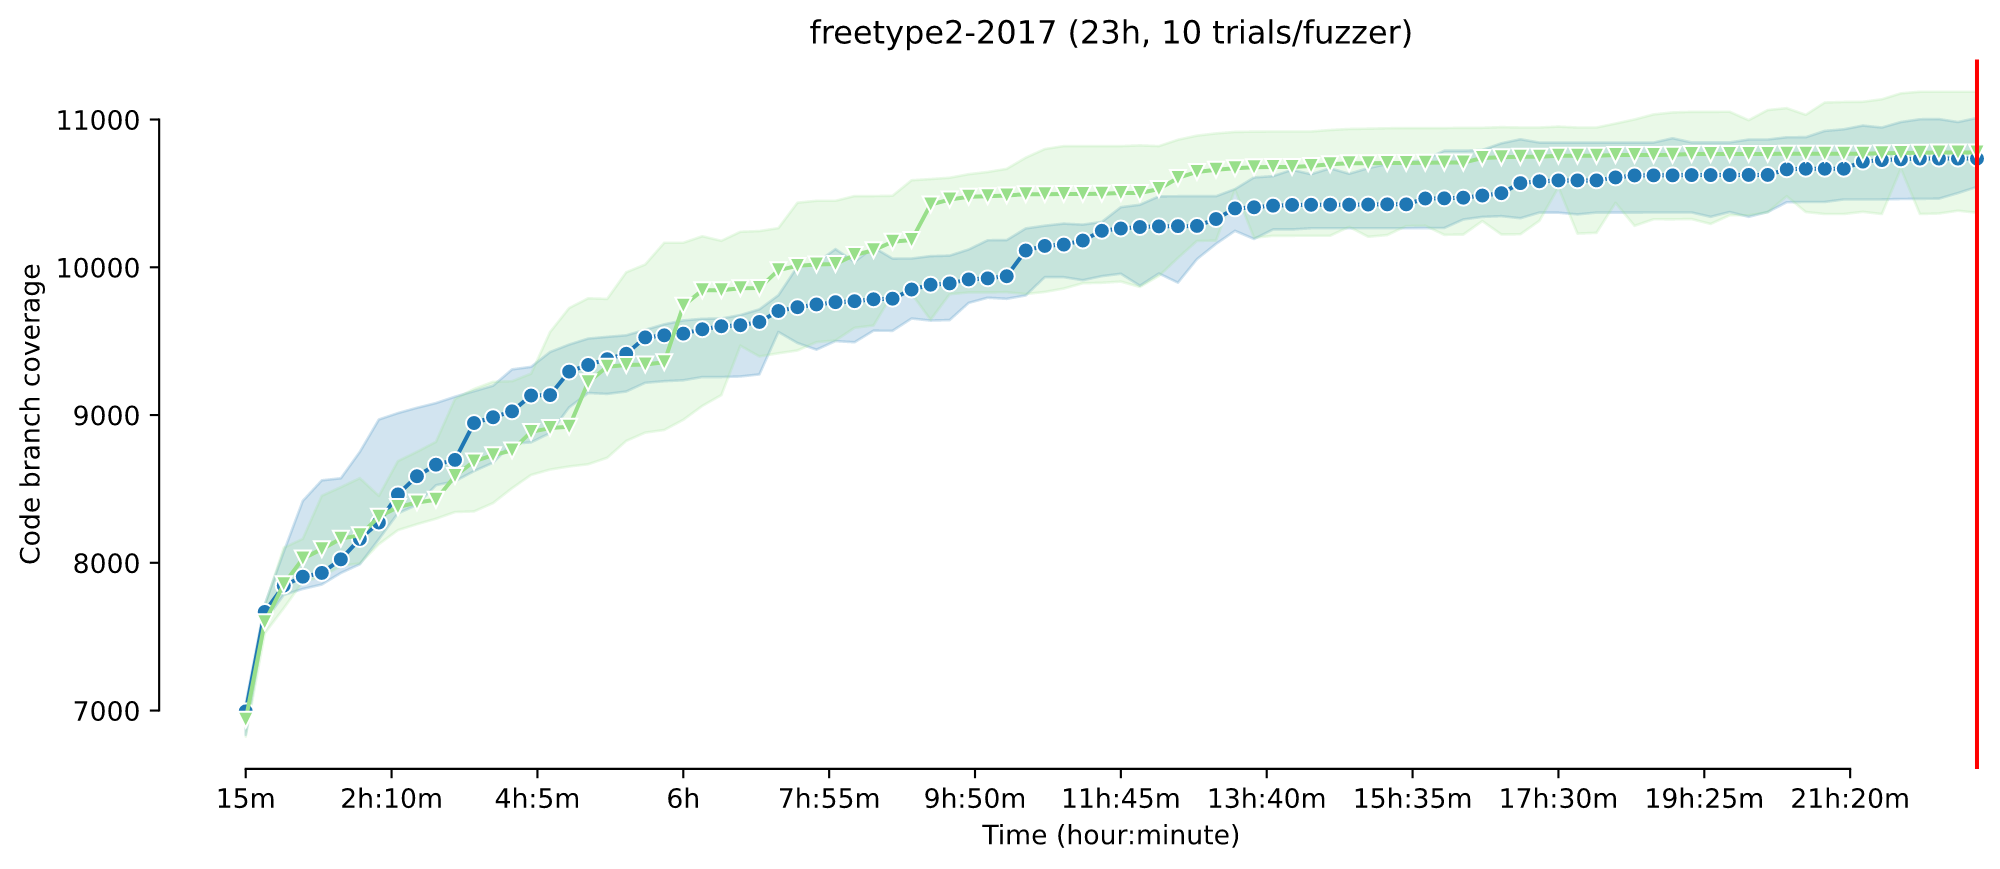
\includegraphics[width=0.65\textwidth]{assets/fuzzbench/symptr-15-1/freetype2-2017_coverage_growth.png}  & 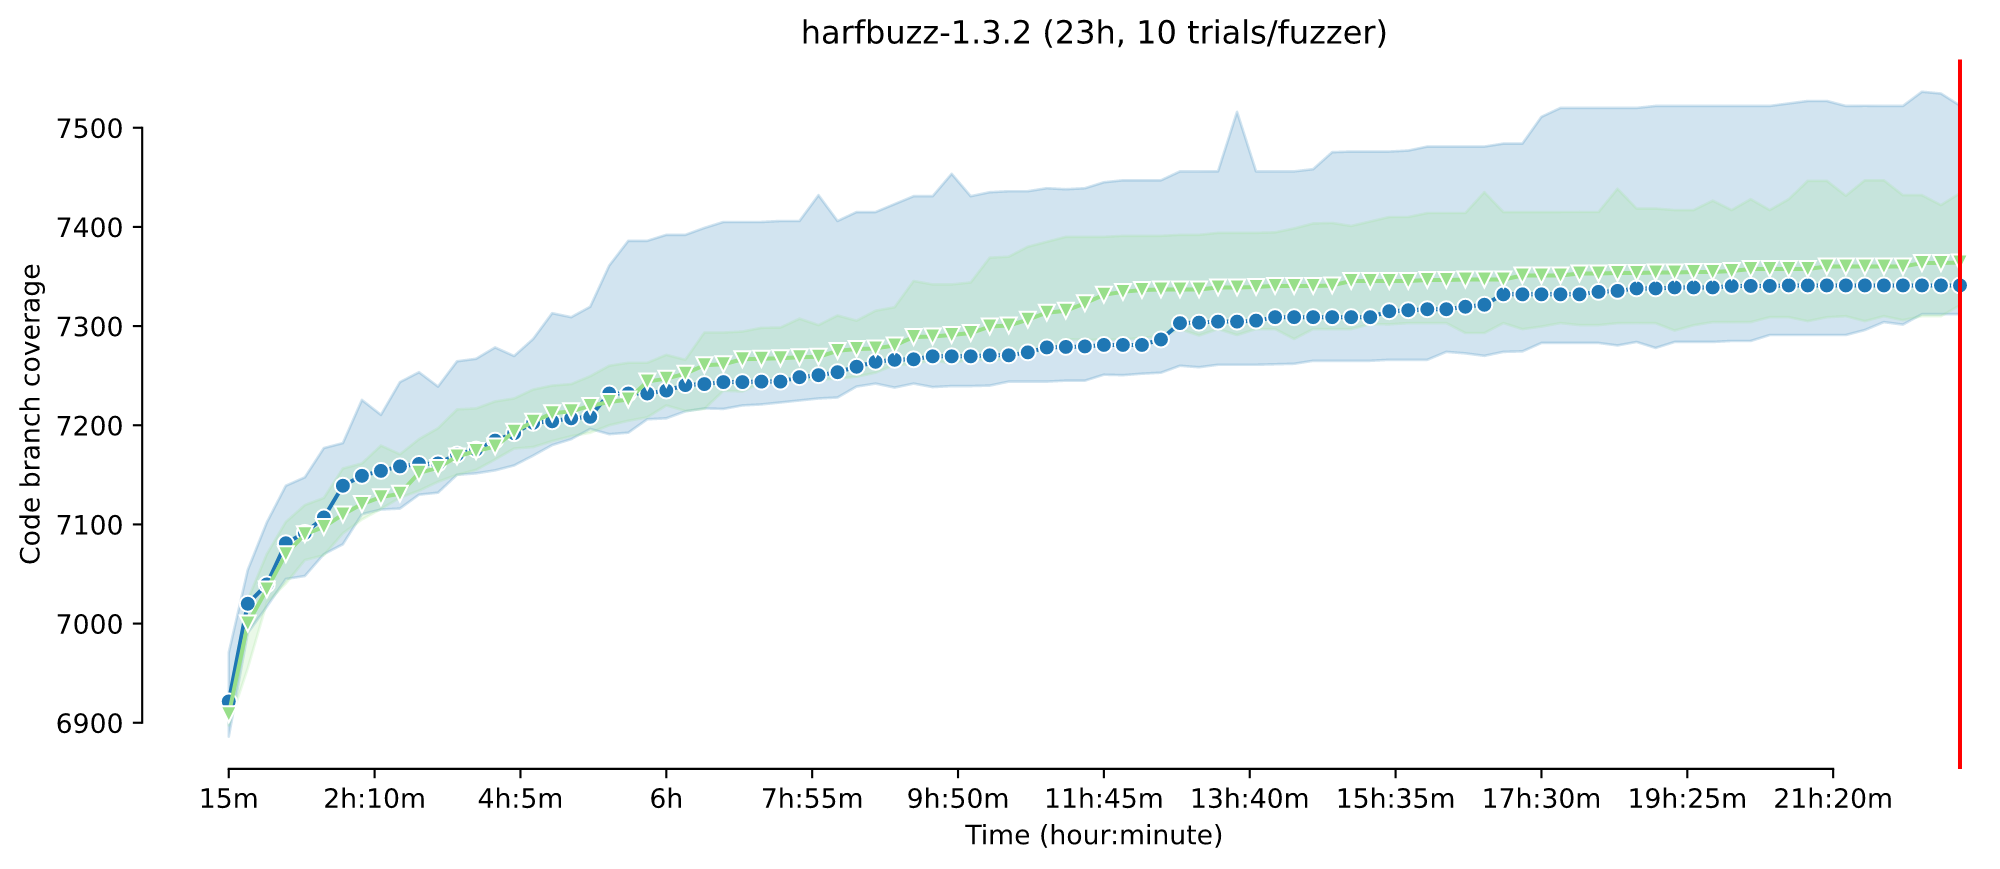
\includegraphics[width=0.65\textwidth]{assets/fuzzbench/symptr-15-1/harfbuzz-1.3.2_coverage_growth.png}        \\
            (a) freetype2                                                                                            & (b) harfbuzz                                                                                                   \\[6pt]
            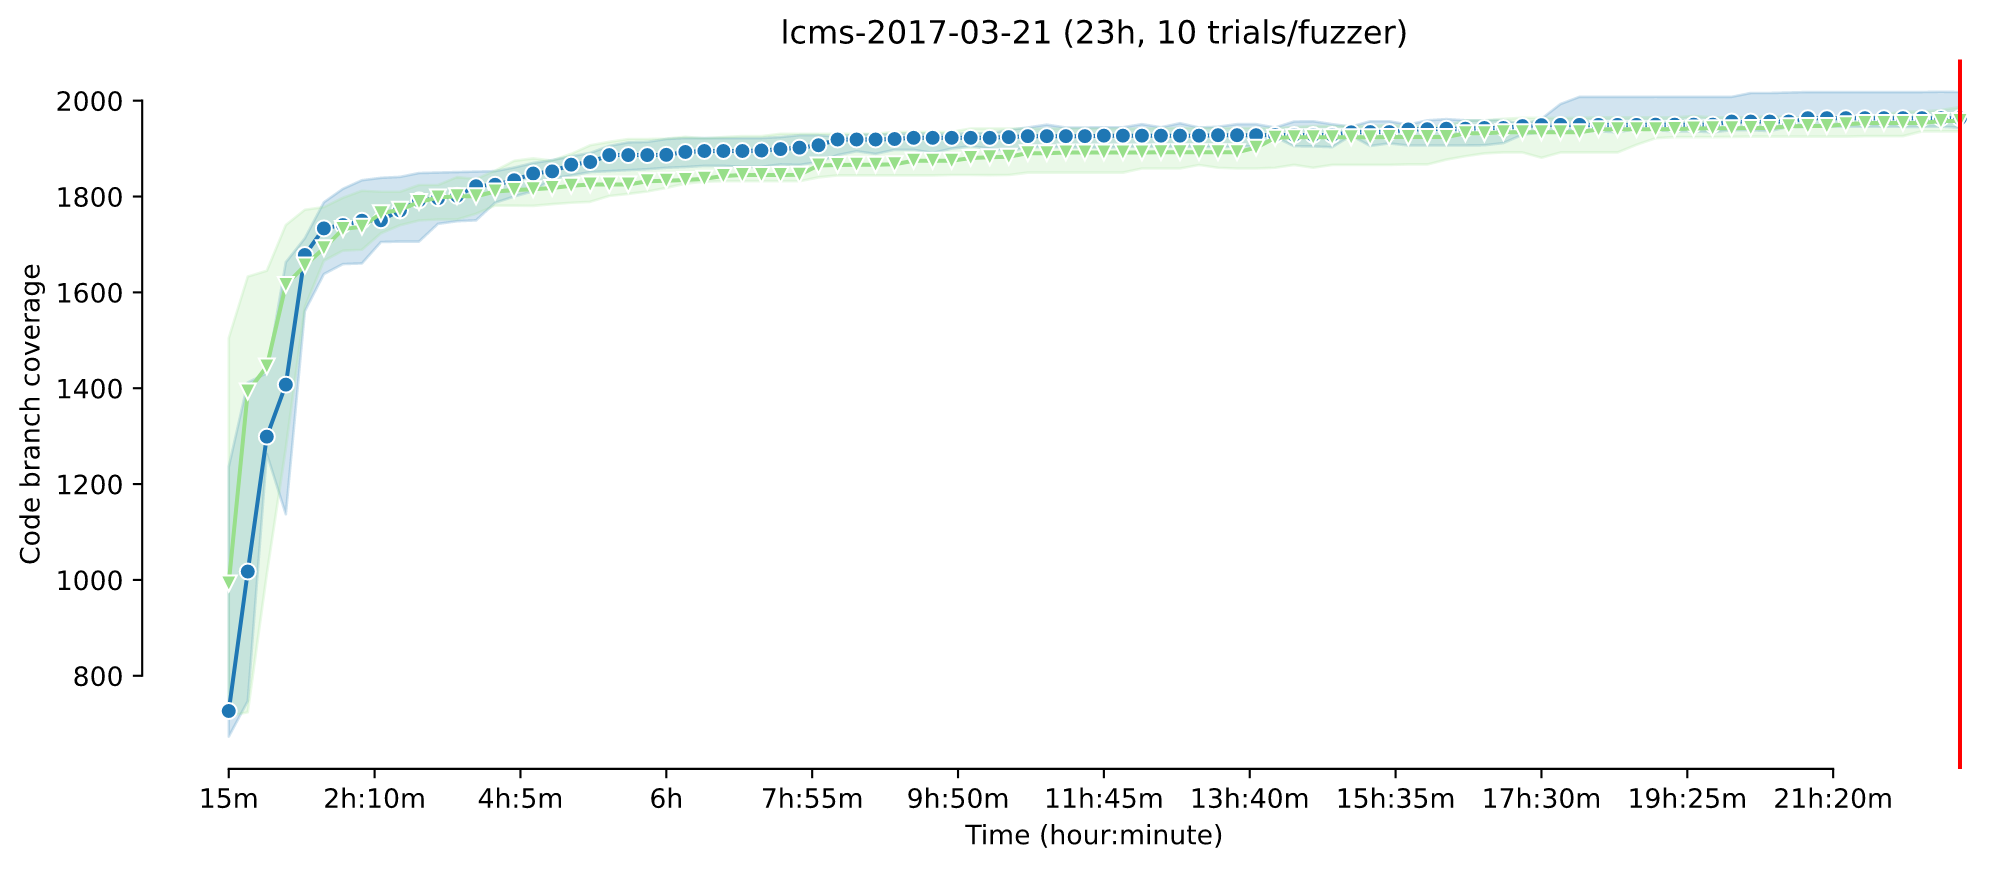
\includegraphics[width=0.65\textwidth]{assets/fuzzbench/symptr-15-1/lcms-2017-03-21_coverage_growth.png} & 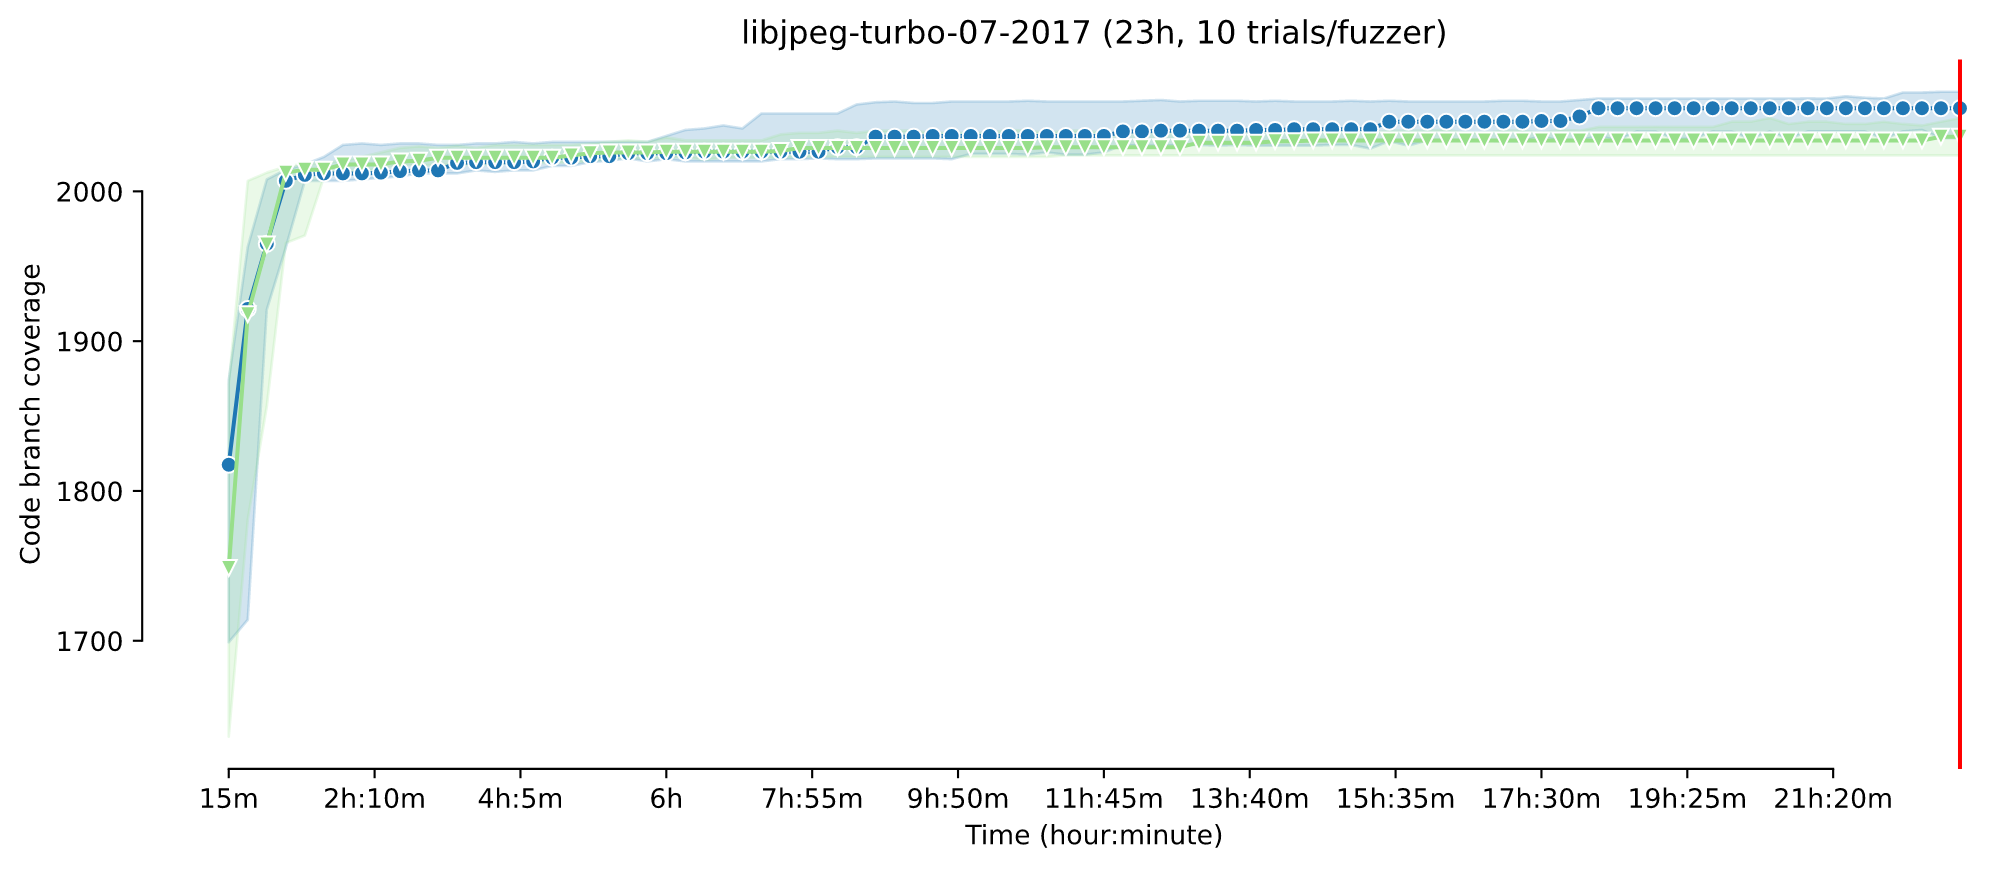
\includegraphics[width=0.65\textwidth]{assets/fuzzbench/symptr-15-1/libjpeg-turbo-07-2017_coverage_growth.png} \\
            (c) lcms                                                                                                 & (d) libjpeg                                                                                                    \\[6pt]
            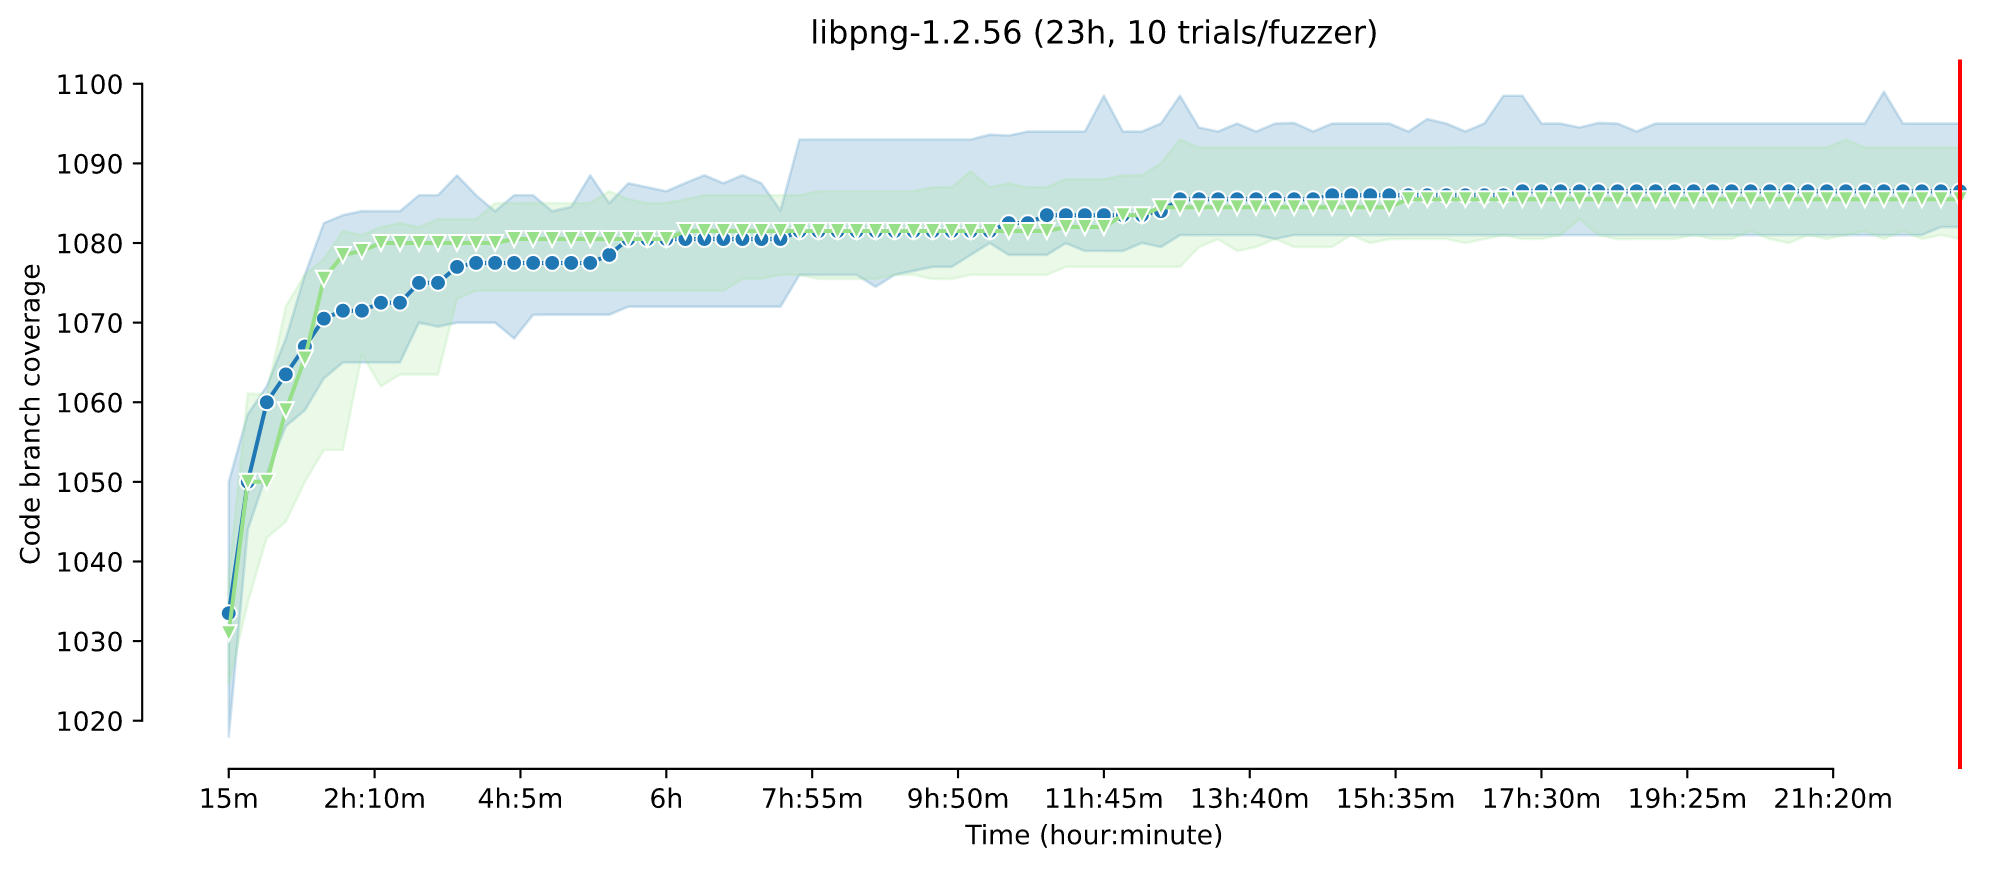
\includegraphics[width=0.65\textwidth]{assets/fuzzbench/symptr-15-1/libpng-1.2.56_coverage_growth.png}   & 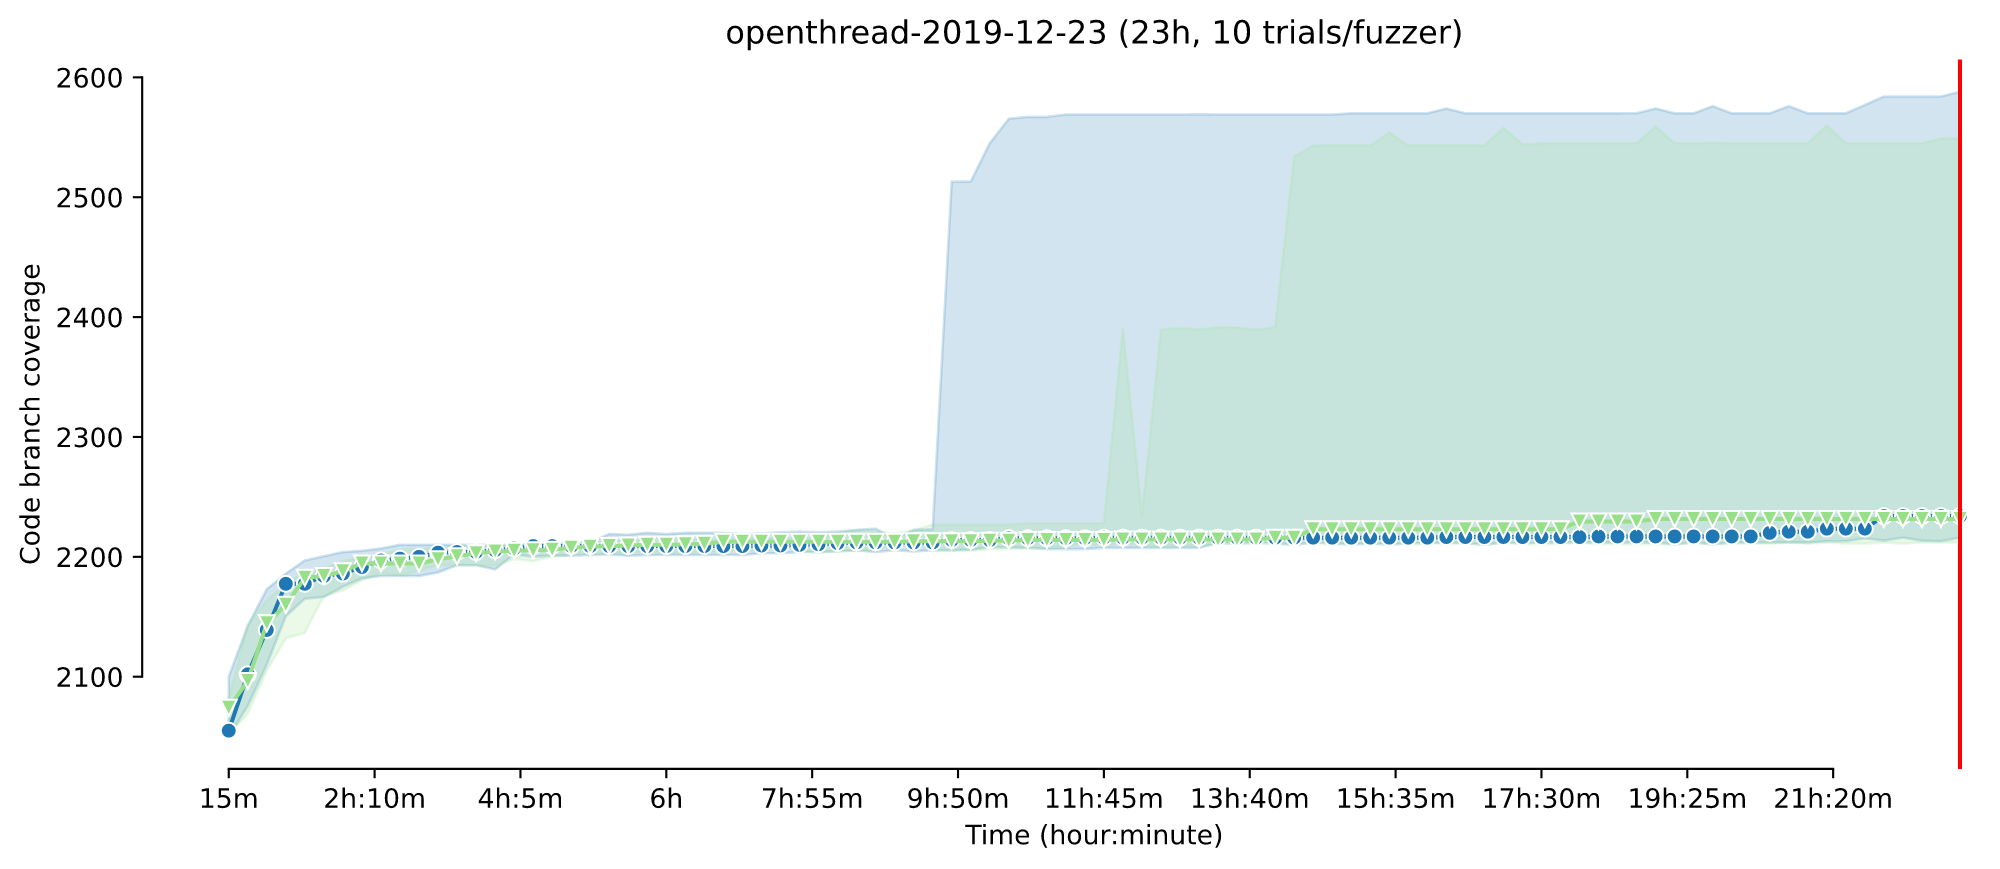
\includegraphics[width=0.65\textwidth]{assets/fuzzbench/symptr-15-1/openthread-2019-12-23_coverage_growth.png} \\
            (c) libpng                                                                                               & (d) openthread                                                                                                 \\[6pt]
            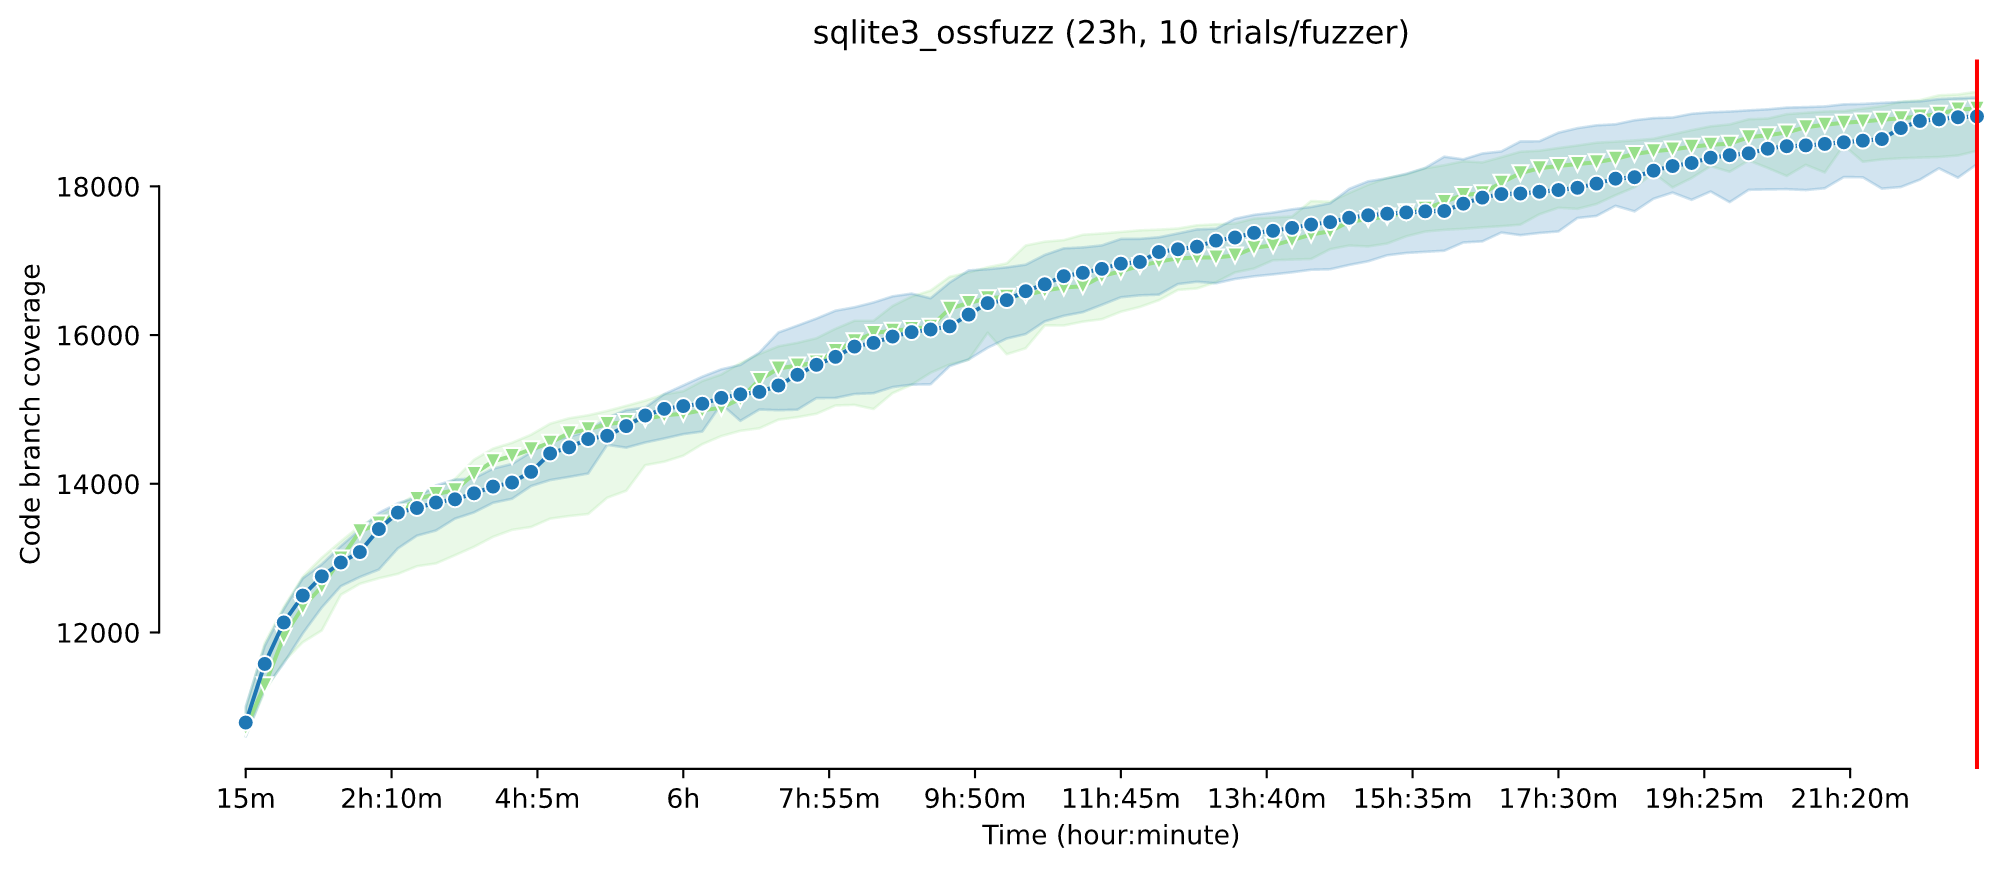
\includegraphics[width=0.65\textwidth]{assets/fuzzbench/symptr-15-1/sqlite3_ossfuzz_coverage_growth.png} & \includegraphics[width=0.65\textwidth]{assets/fuzzbench/symptr-15-1/fuzzbench-legend.png}                      \\
            (c) sqlite3                                                                                              & (d) legend                                                                                                     \\[6pt]
        \end{tabular}
    }
    \caption{Fuzzbench: Symptr-15-1 coverage growth.}
    \label{fig:fuzzbench:symptr-15-1}
\end{figure}

\begin{figure}[t]
    \centering
    \resizebox{\columnwidth}{!}{%
        \begin{tabular}{cc}
            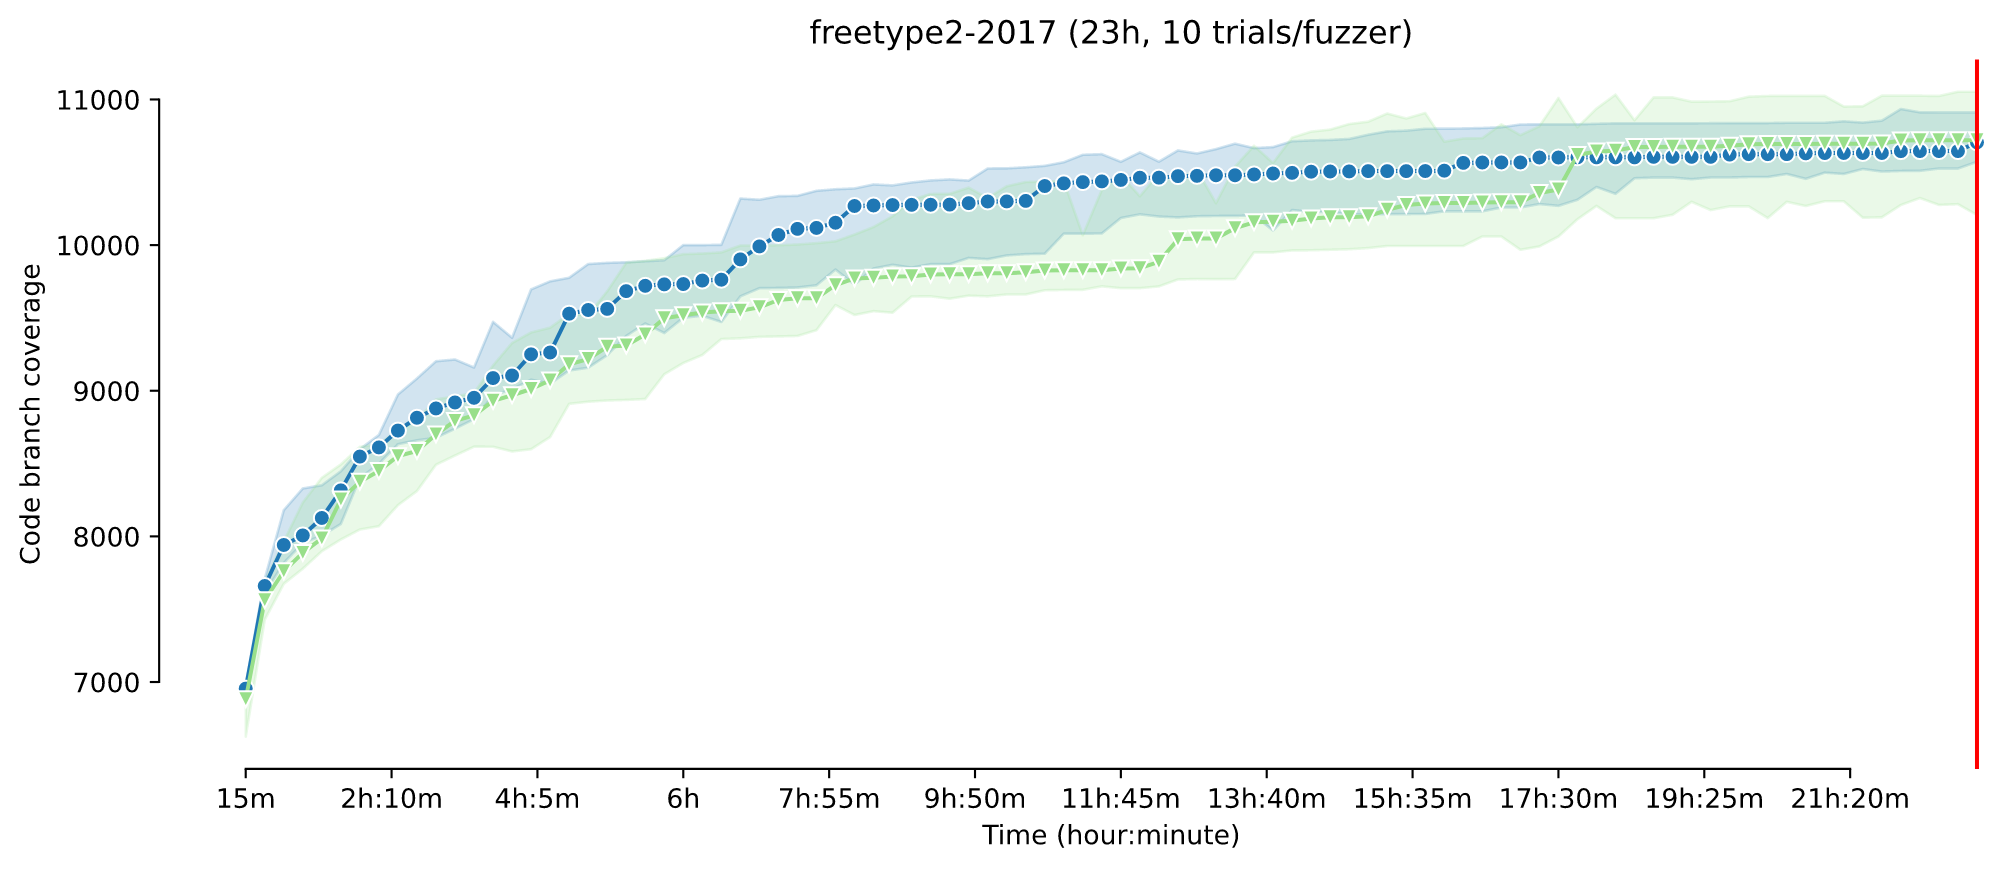
\includegraphics[width=0.65\textwidth]{assets/fuzzbench/symptr-25-1/freetype2-2017_coverage_growth.png}  & 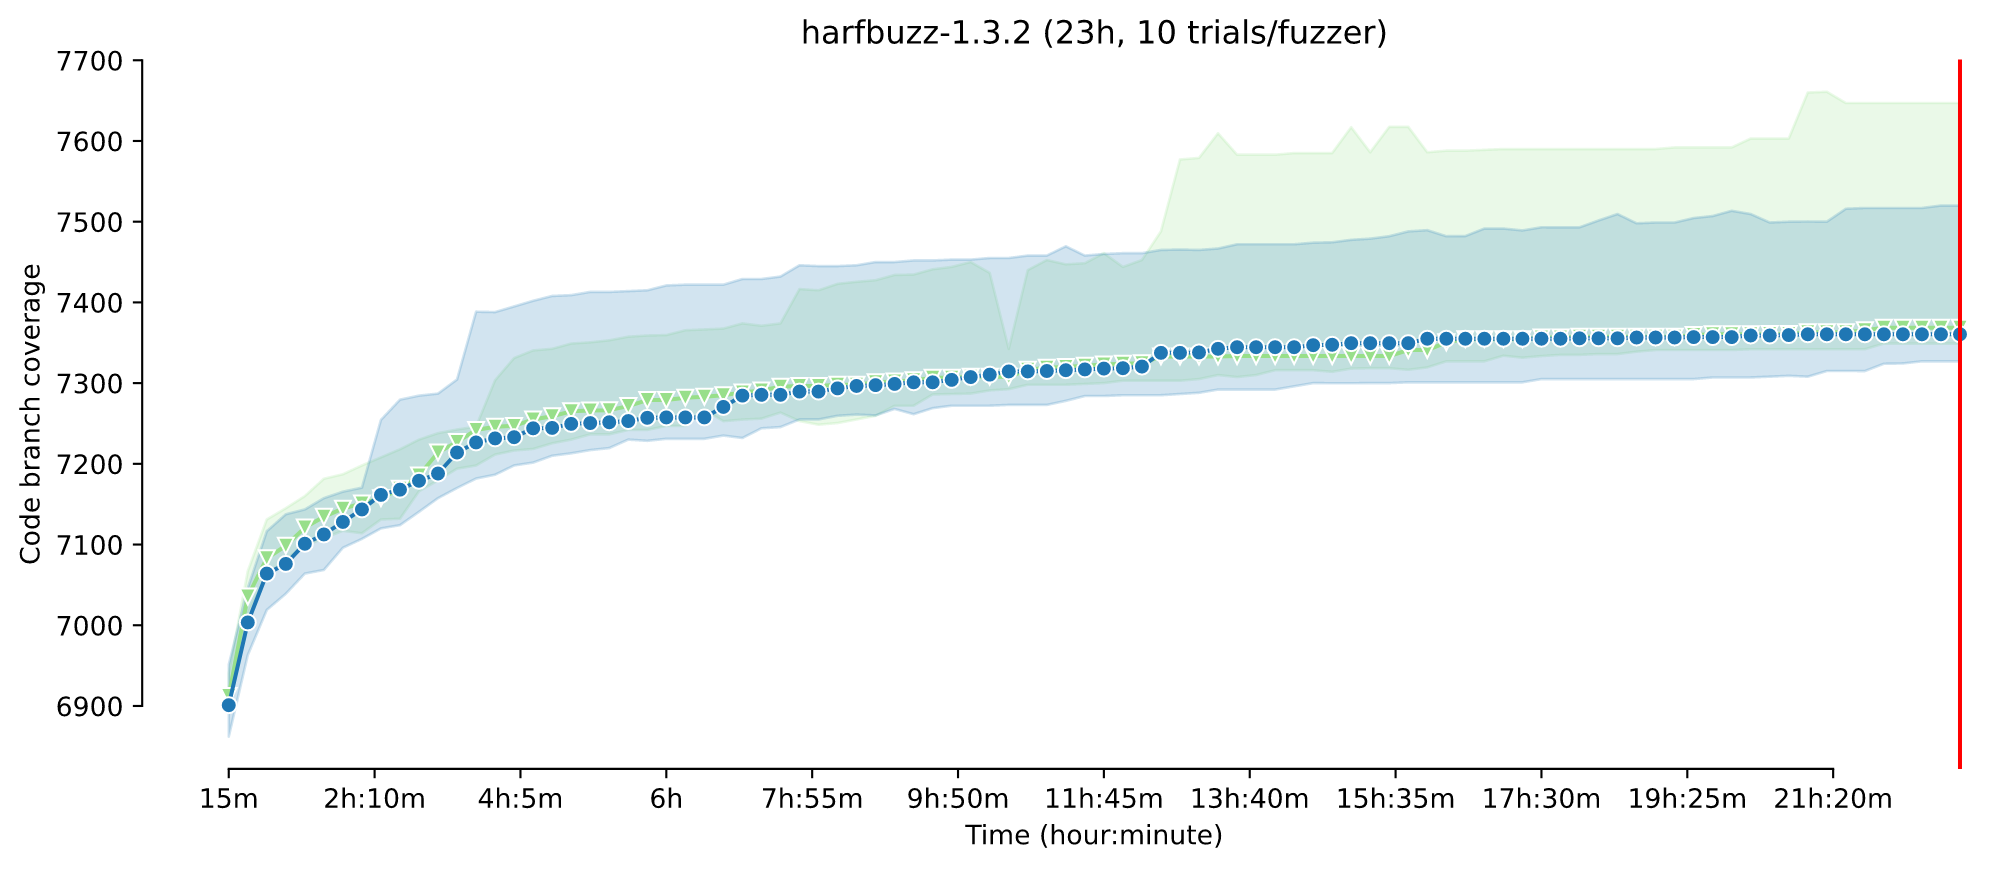
\includegraphics[width=0.65\textwidth]{assets/fuzzbench/symptr-25-1/harfbuzz-1.3.2_coverage_growth.png}        \\
            (a) freetype2                                                                                            & (b) harfbuzz                                                                                                   \\[6pt]
            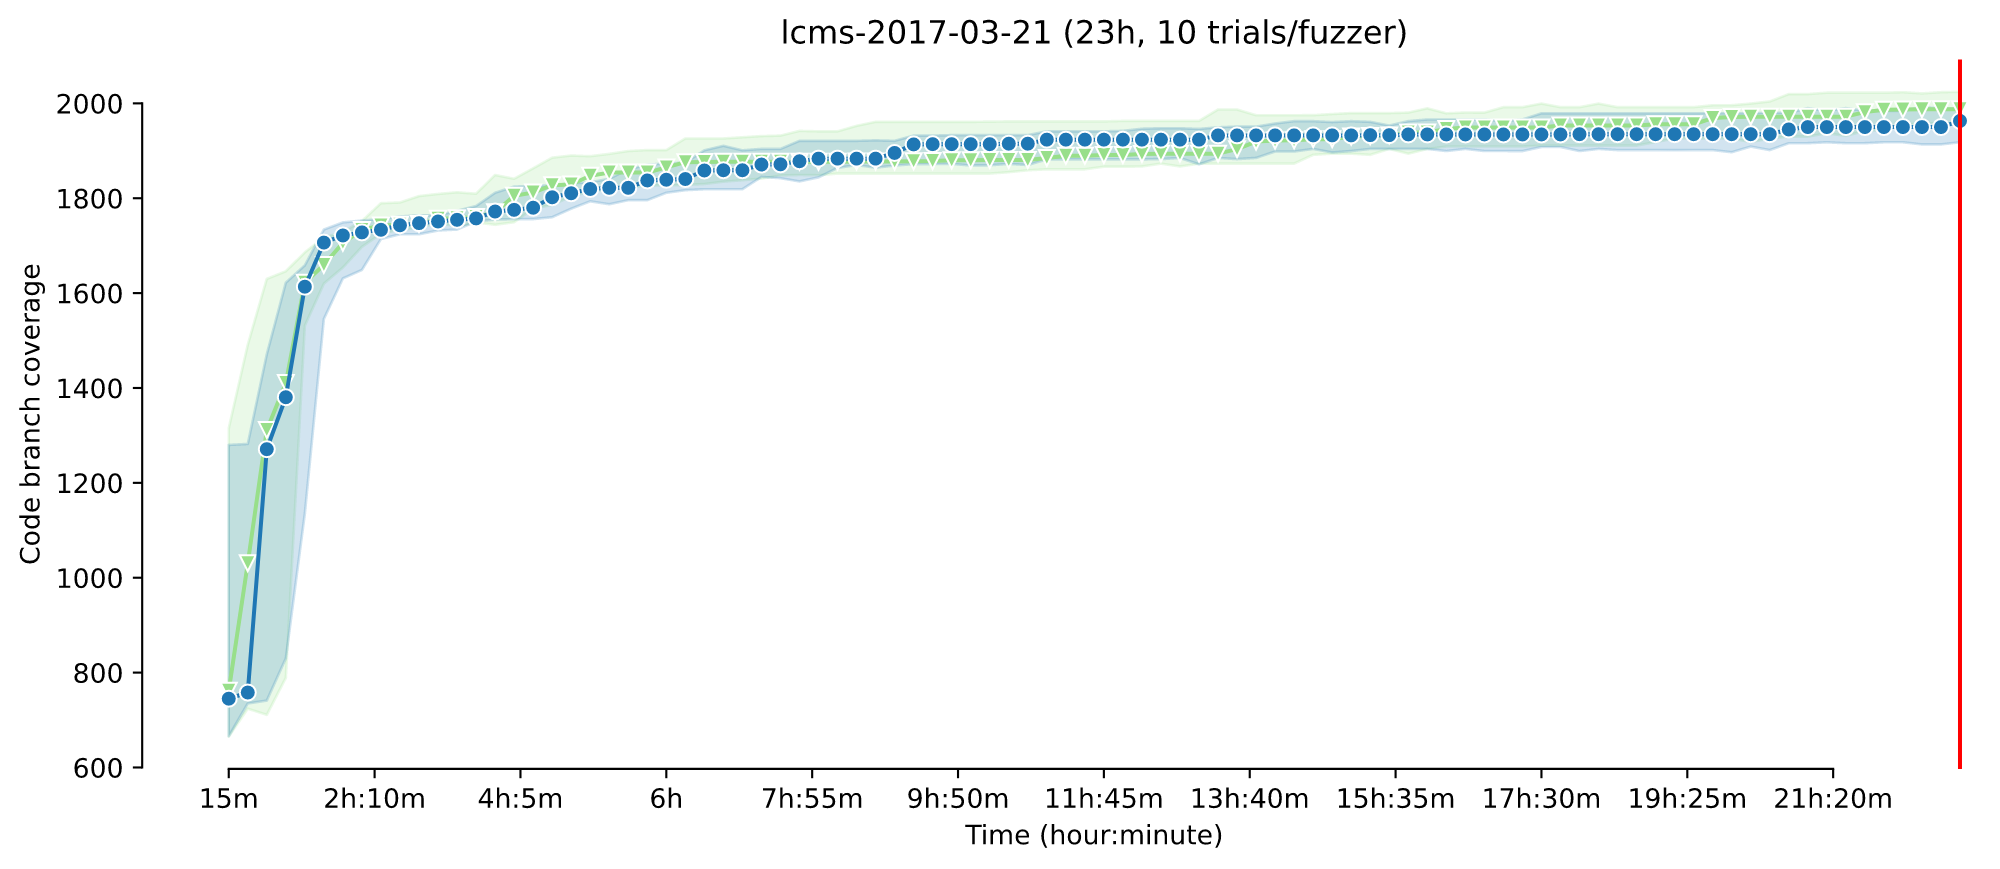
\includegraphics[width=0.65\textwidth]{assets/fuzzbench/symptr-25-1/lcms-2017-03-21_coverage_growth.png} & 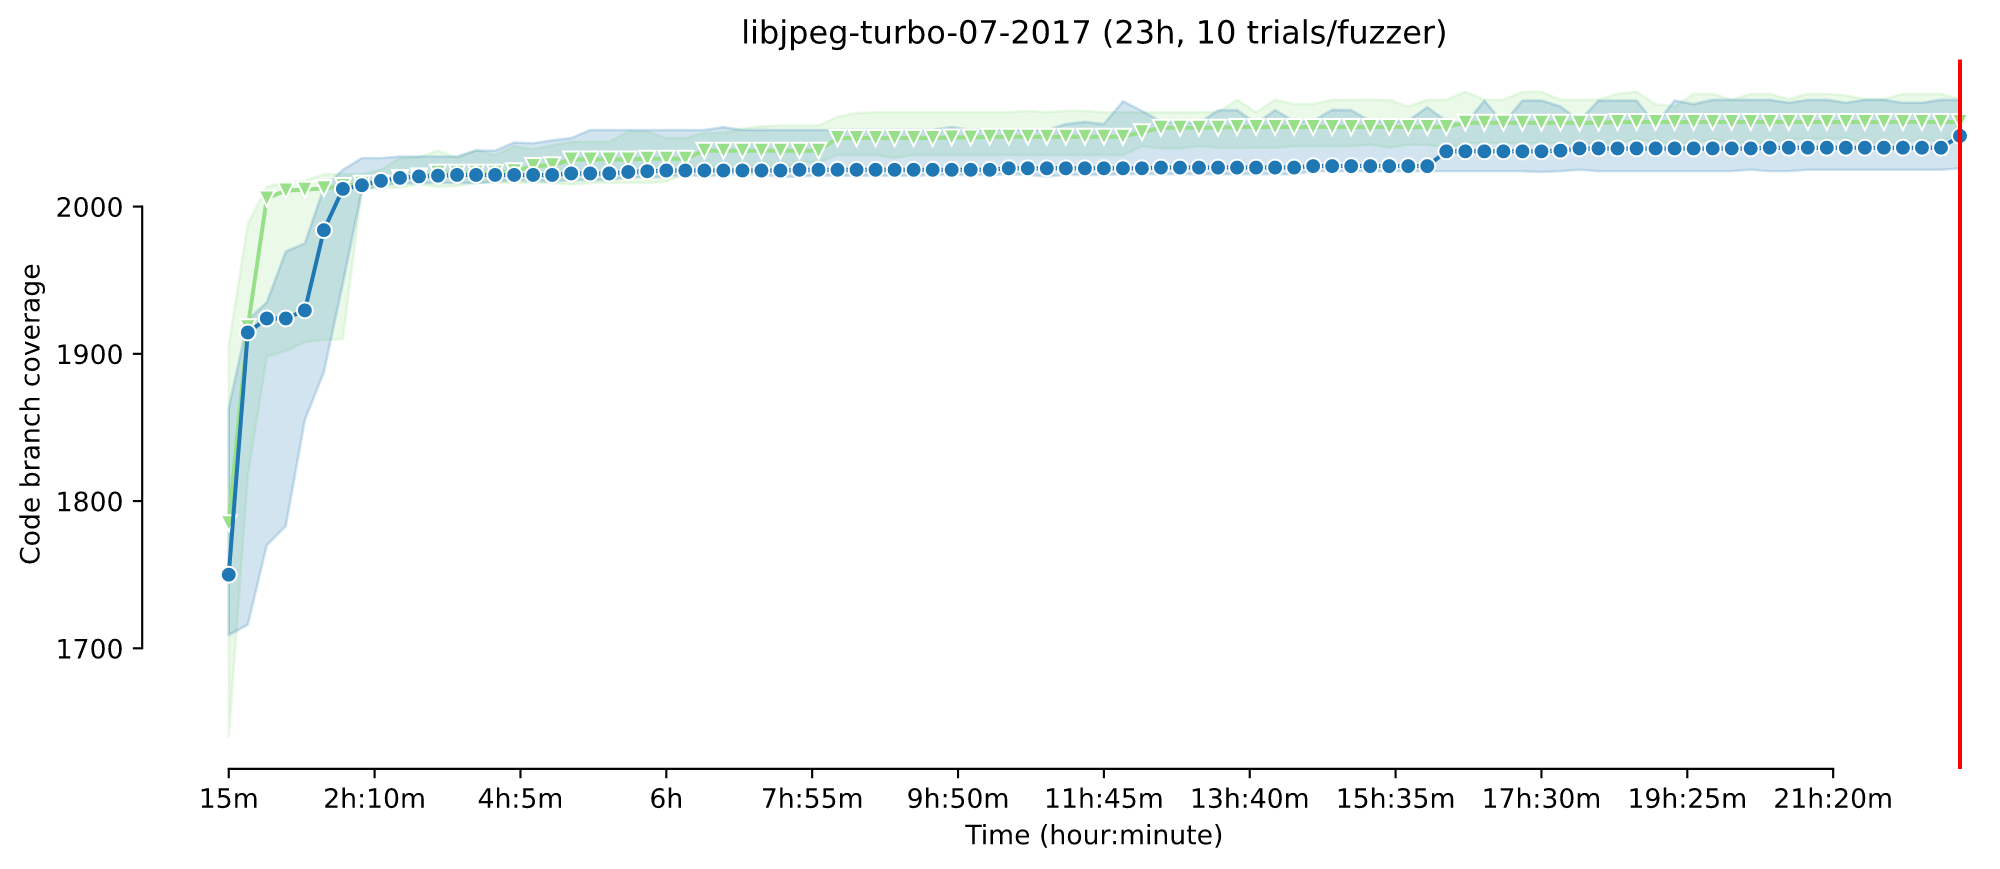
\includegraphics[width=0.65\textwidth]{assets/fuzzbench/symptr-25-1/libjpeg-turbo-07-2017_coverage_growth.png} \\
            (c) lcms                                                                                                 & (d) libjpeg                                                                                                    \\[6pt]
            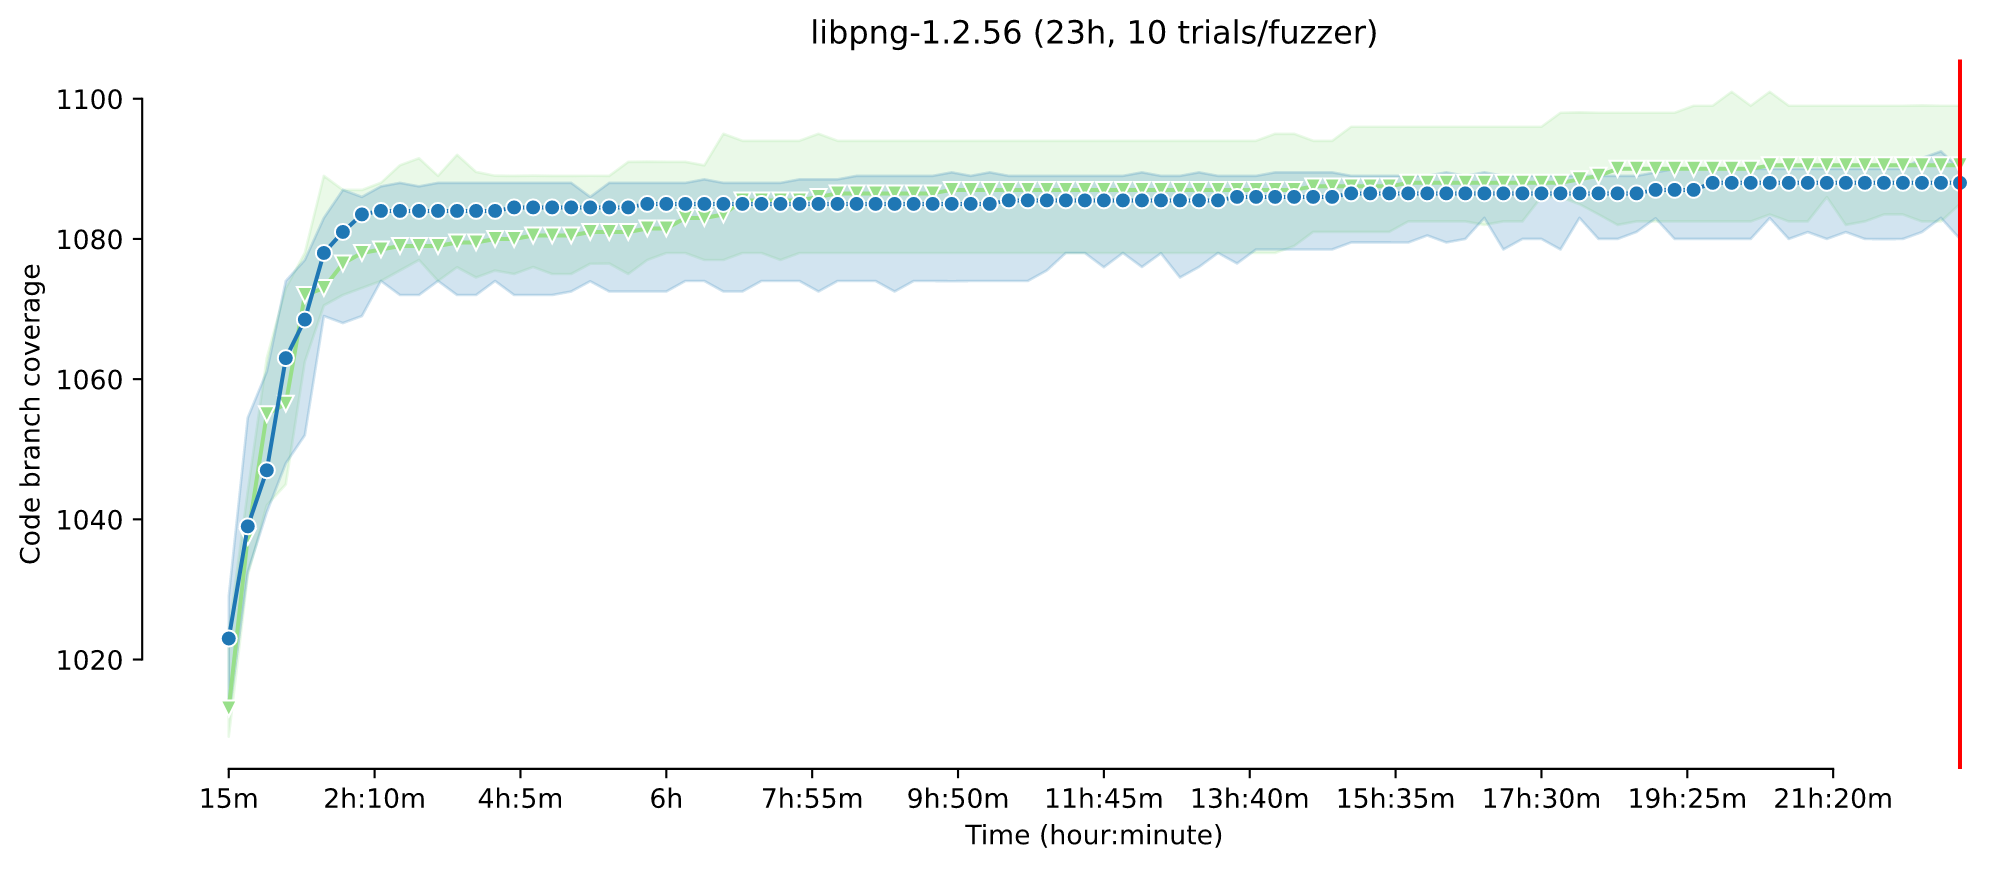
\includegraphics[width=0.65\textwidth]{assets/fuzzbench/symptr-25-1/libpng-1.2.56_coverage_growth.png}   & 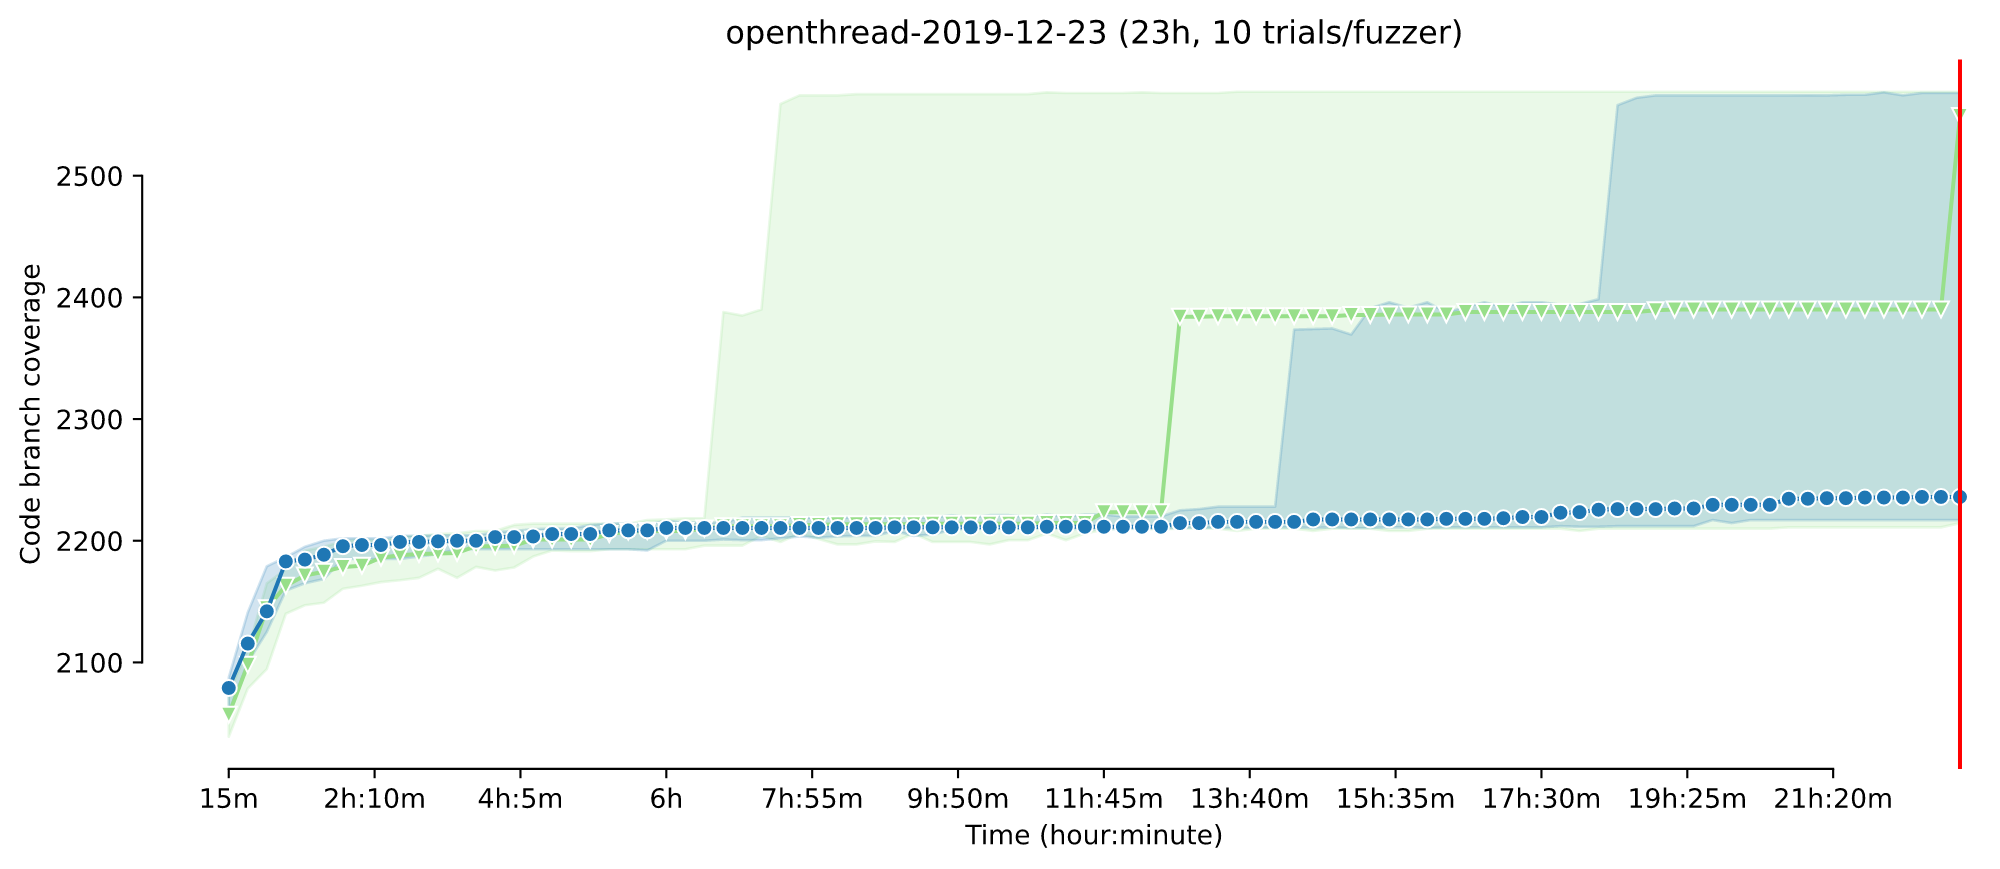
\includegraphics[width=0.65\textwidth]{assets/fuzzbench/symptr-25-1/openthread-2019-12-23_coverage_growth.png} \\
            (c) libpng                                                                                               & (d) openthread                                                                                                 \\[6pt]
            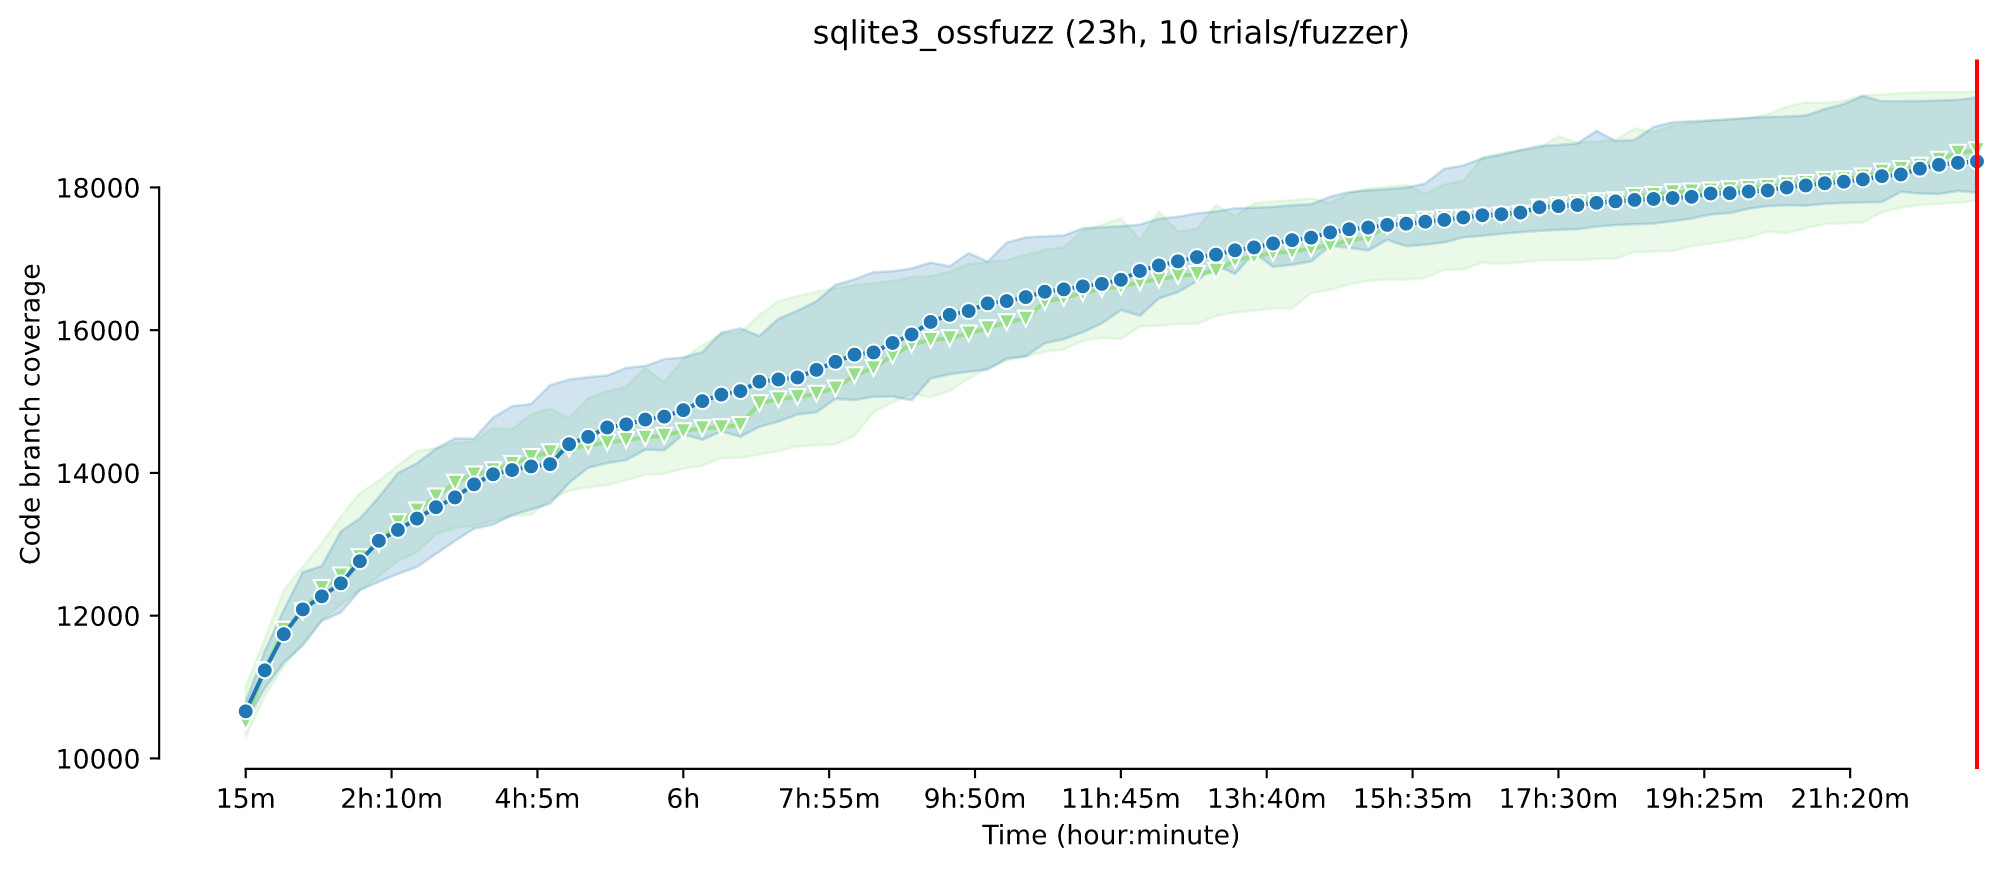
\includegraphics[width=0.65\textwidth]{assets/fuzzbench/symptr-25-1/sqlite3_ossfuzz_coverage_growth.png} & \includegraphics[width=0.65\textwidth]{assets/fuzzbench/symptr-25-1/fuzzbench-legend.png}                      \\
            (c) sqlite3                                                                                              & (d) legend                                                                                                     \\[6pt]
        \end{tabular}
    }
    \caption{Fuzzbench: Symptr-25-1 coverage growth.}
    \label{fig:fuzzbench:symptr-25-1}
\end{figure}

\begin{figure}[t]
    \centering
    \resizebox{\columnwidth}{!}{%
        \begin{tabular}{cc}
            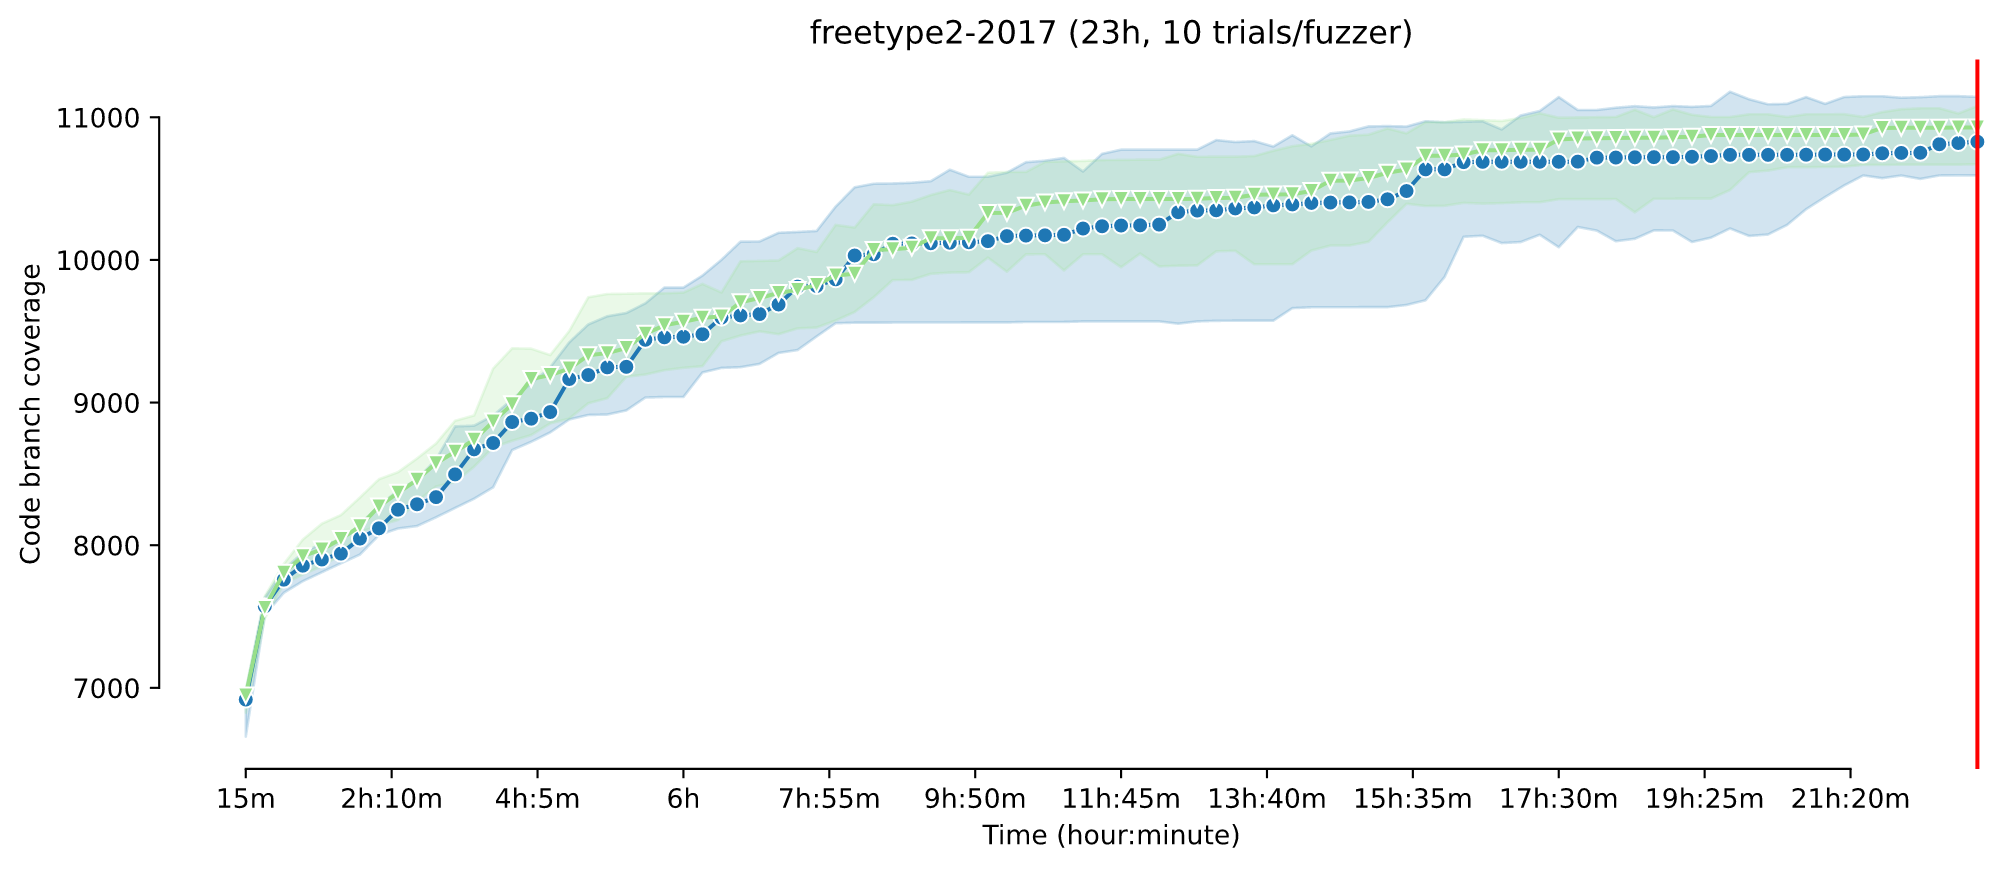
\includegraphics[width=0.65\textwidth]{assets/fuzzbench/symptr-25-vs-35-2/freetype2-2017_coverage_growth.png}  & 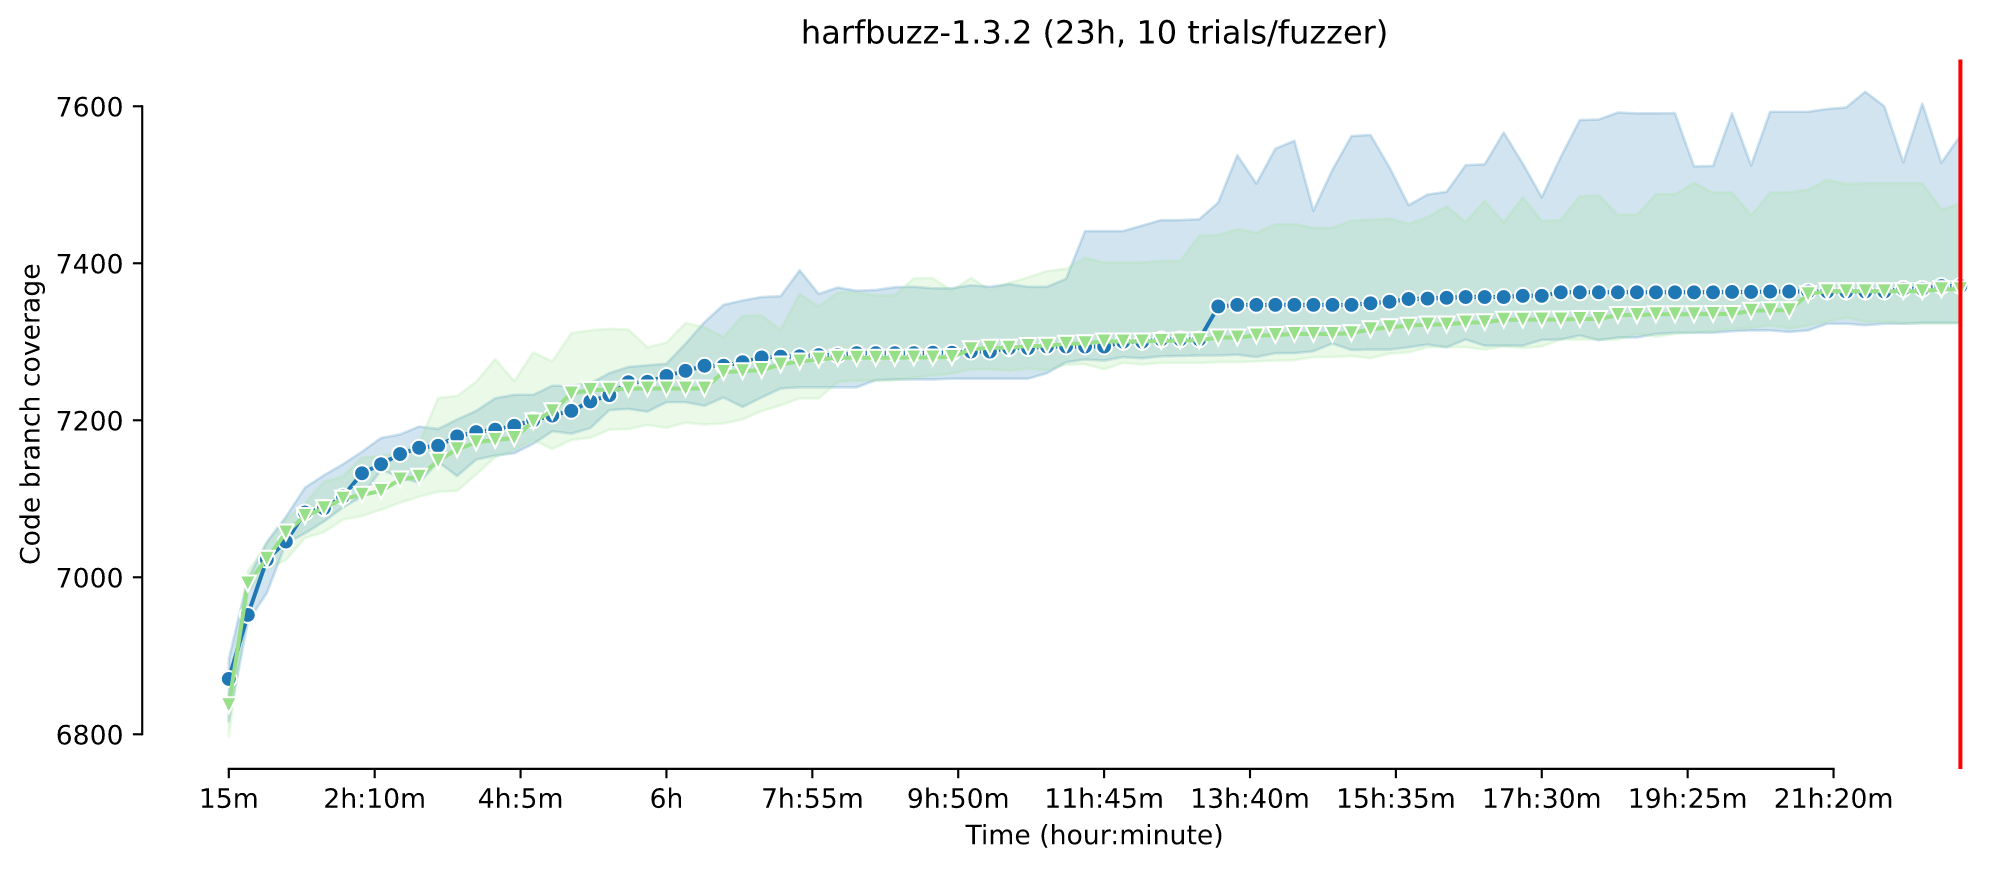
\includegraphics[width=0.65\textwidth]{assets/fuzzbench/symptr-25-vs-35-2/harfbuzz-1.3.2_coverage_growth.png}        \\
            (a) freetype2                                                                                                  & (b) harfbuzz                                                                                                         \\[6pt]
            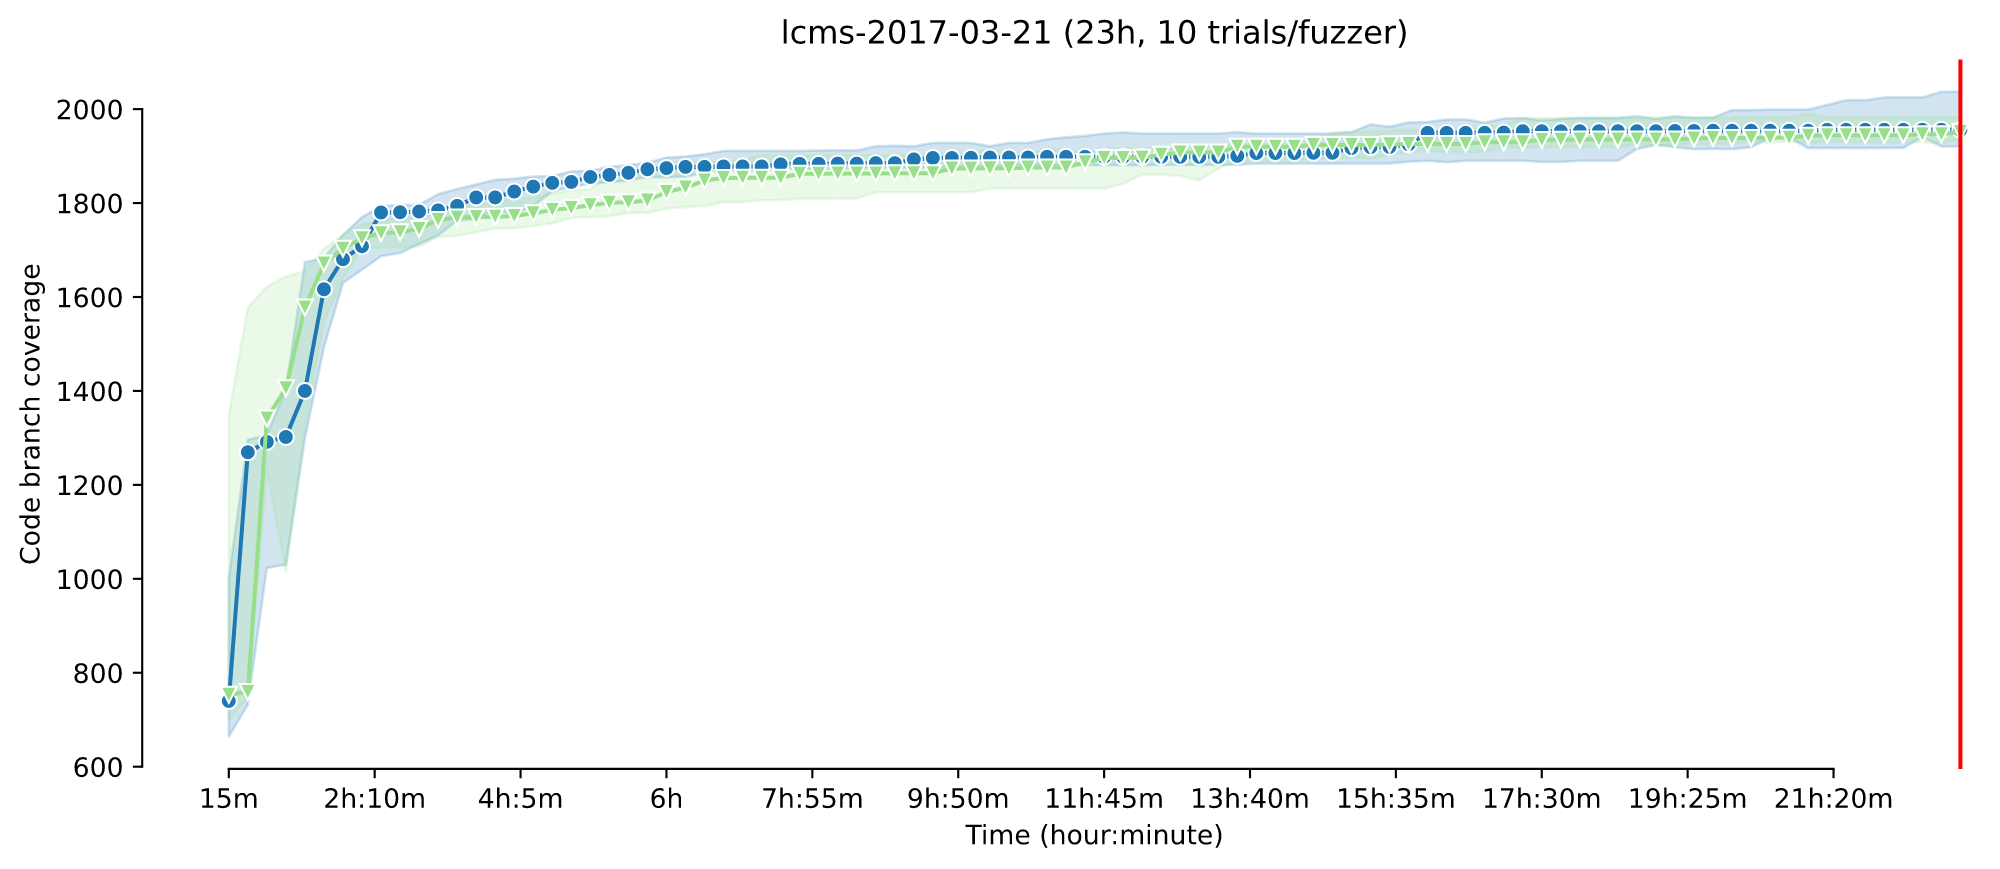
\includegraphics[width=0.65\textwidth]{assets/fuzzbench/symptr-25-vs-35-2/lcms-2017-03-21_coverage_growth.png} & 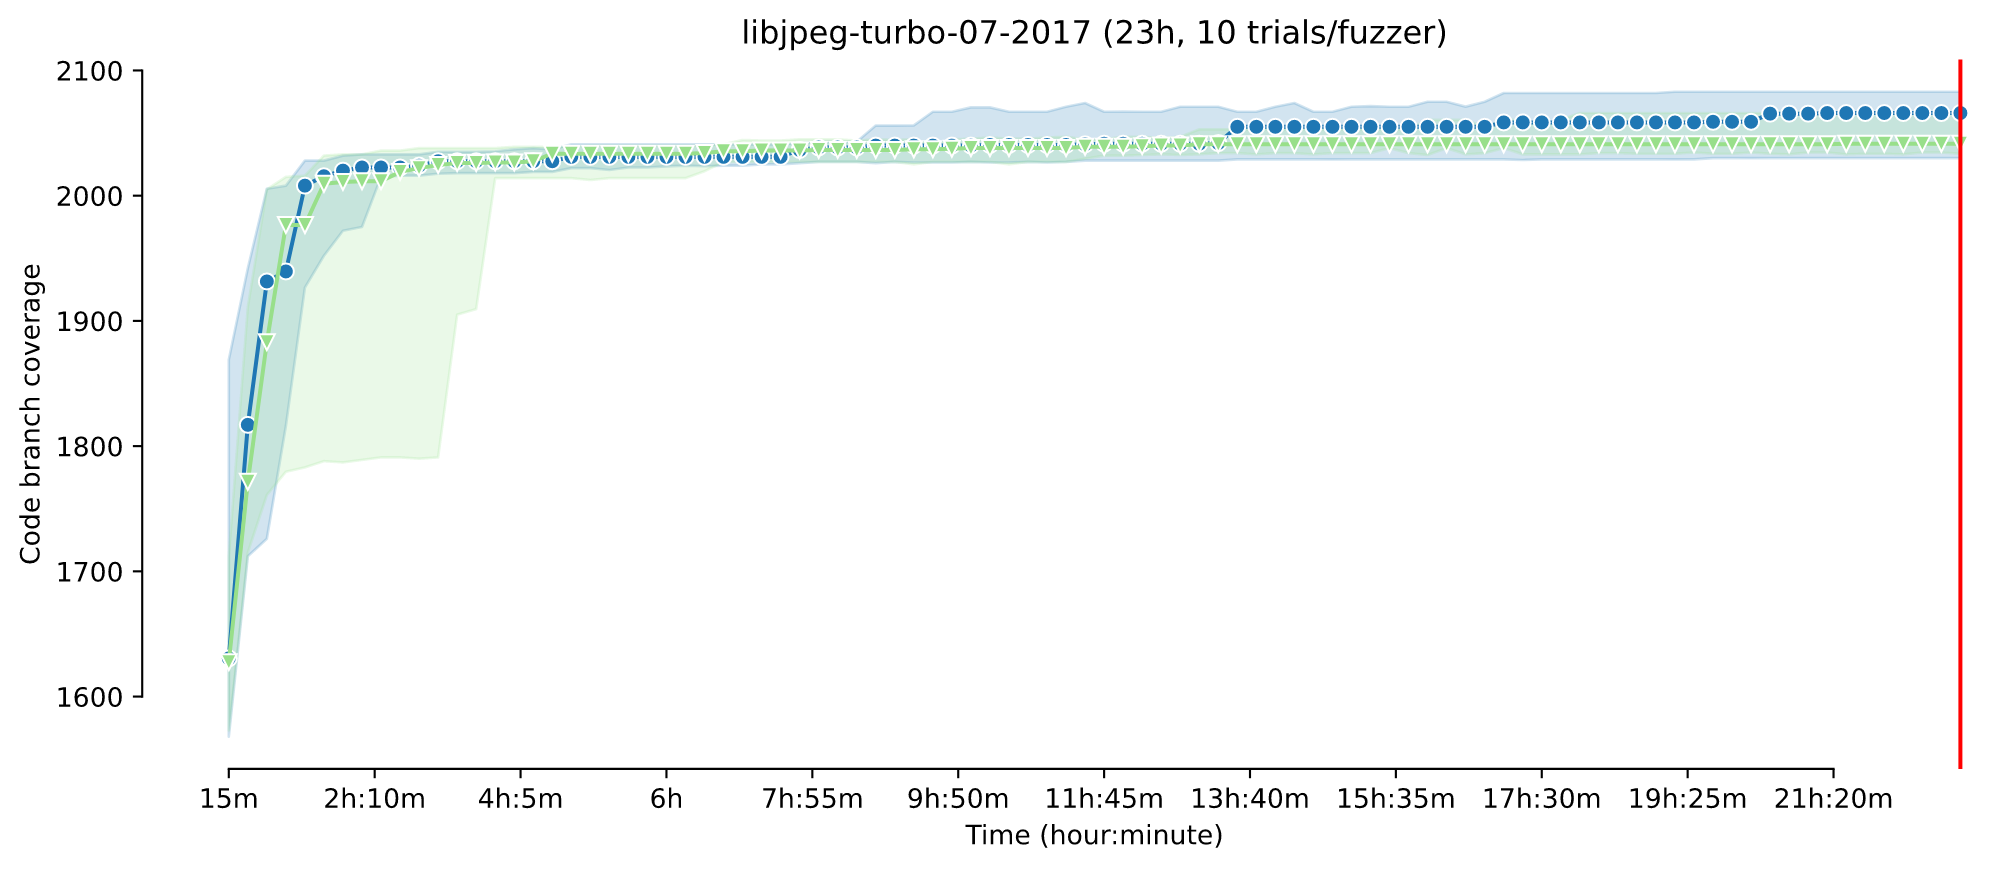
\includegraphics[width=0.65\textwidth]{assets/fuzzbench/symptr-25-vs-35-2/libjpeg-turbo-07-2017_coverage_growth.png} \\
            (c) lcms                                                                                                       & (d) libjpeg                                                                                                          \\[6pt]
            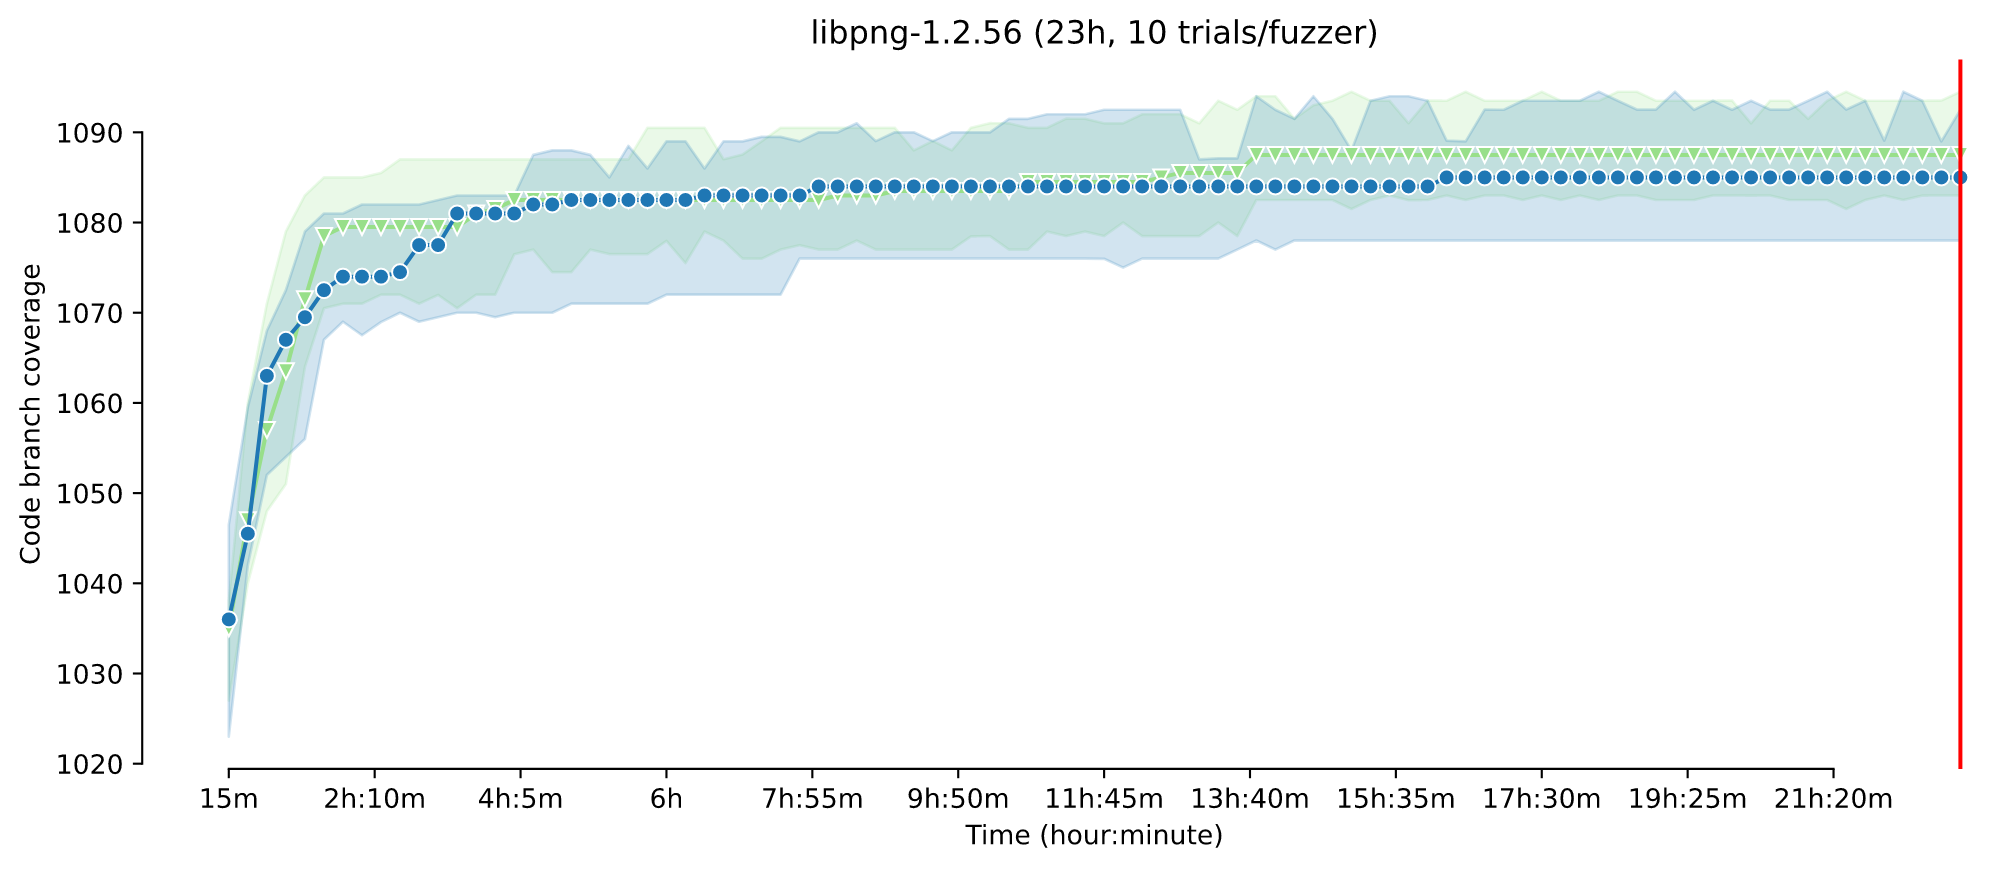
\includegraphics[width=0.65\textwidth]{assets/fuzzbench/symptr-25-vs-35-2/libpng-1.2.56_coverage_growth.png}   & 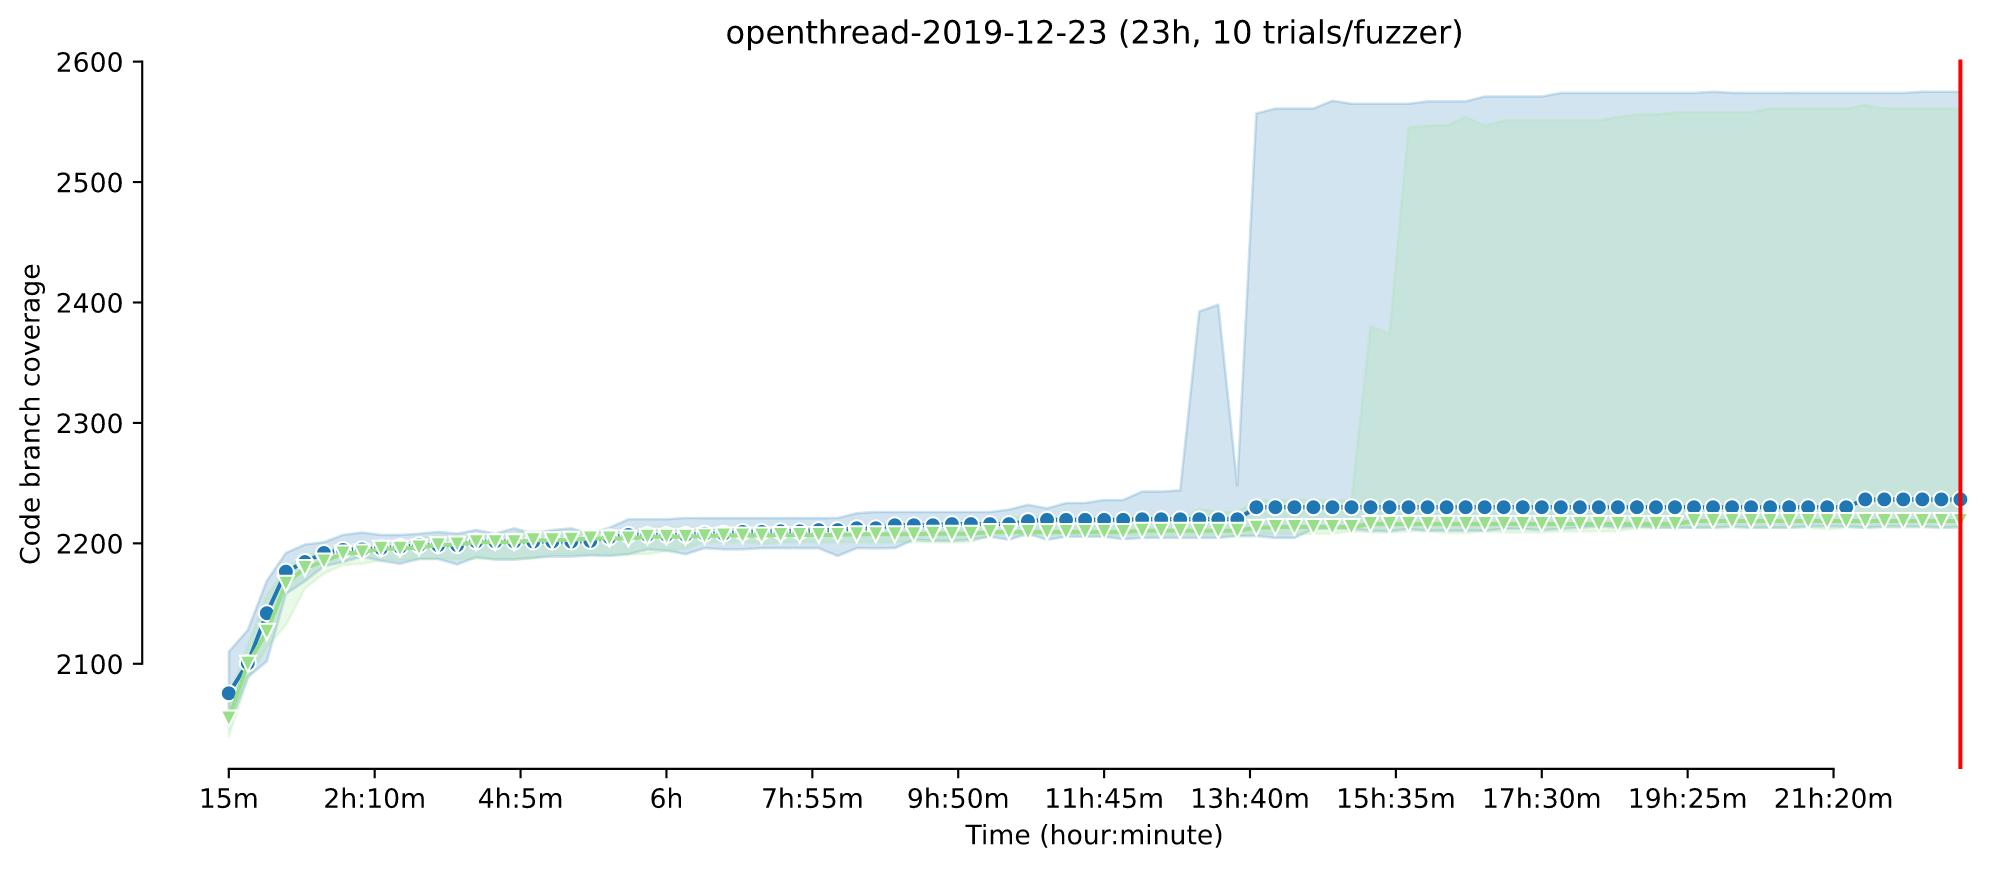
\includegraphics[width=0.65\textwidth]{assets/fuzzbench/symptr-25-vs-35-2/openthread-2019-12-23_coverage_growth.png} \\
            (c) libpng                                                                                                     & (d) openthread                                                                                                       \\[6pt]
            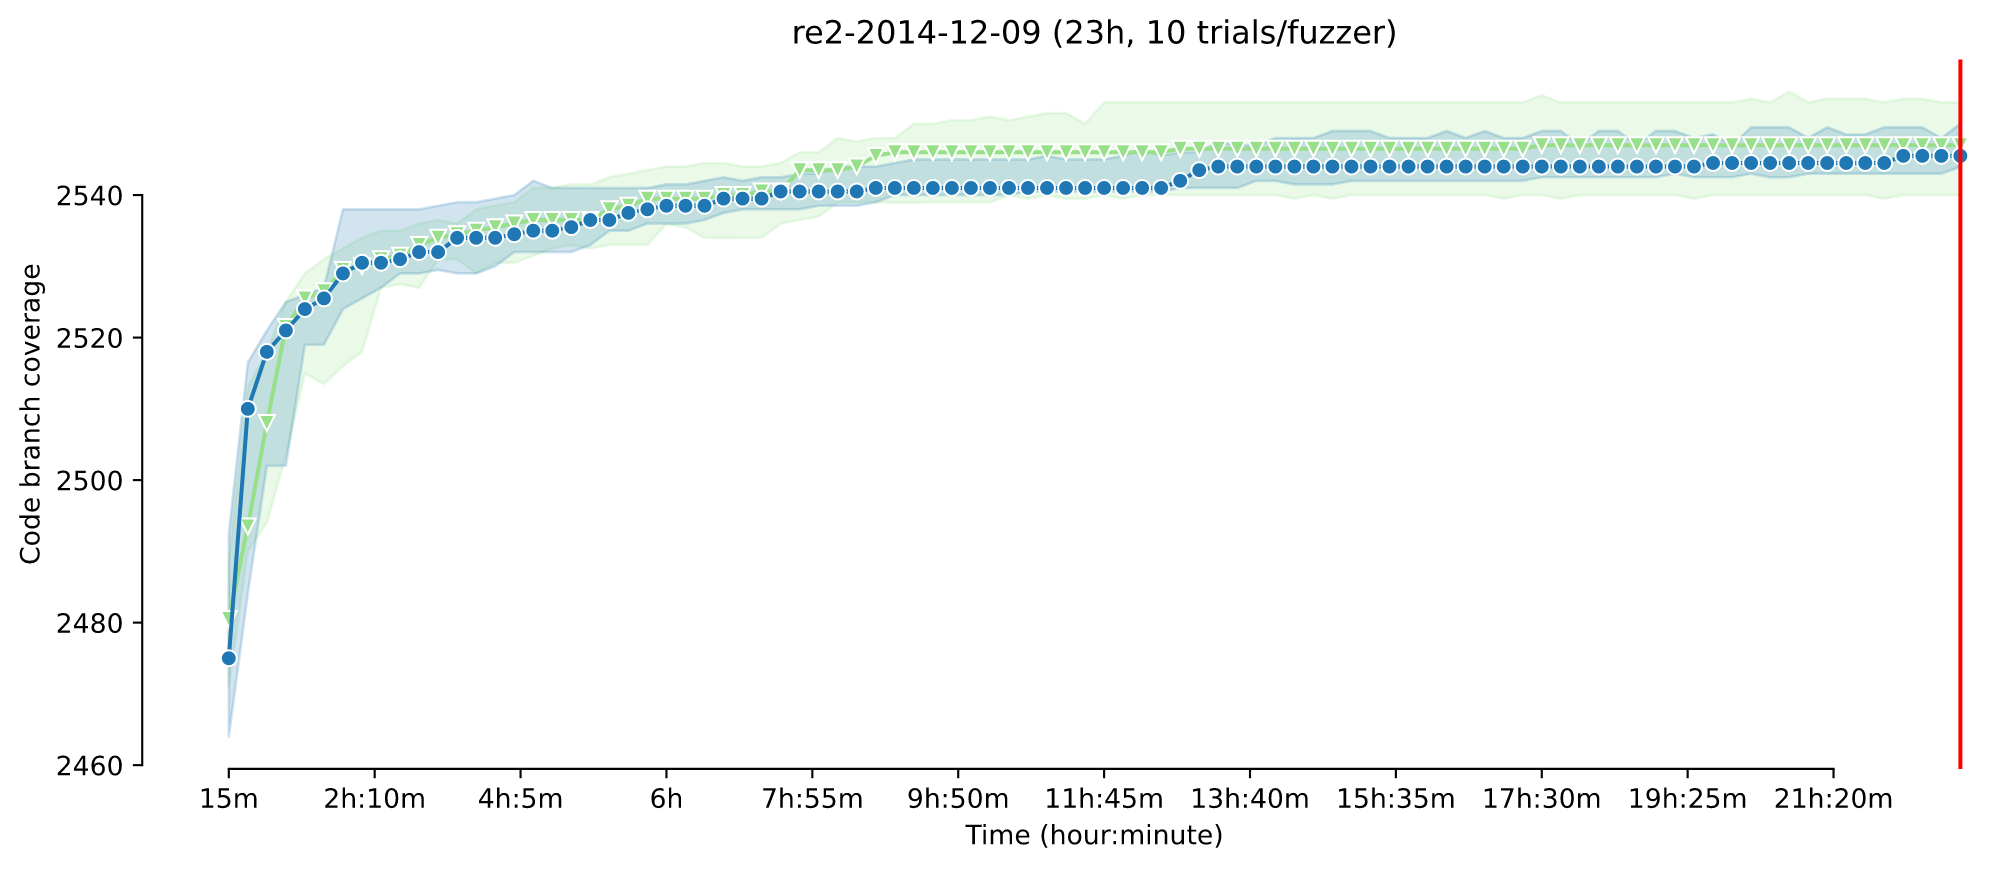
\includegraphics[width=0.65\textwidth]{assets/fuzzbench/symptr-25-vs-35-2/re2-2014-12-09_coverage_growth.png}  & 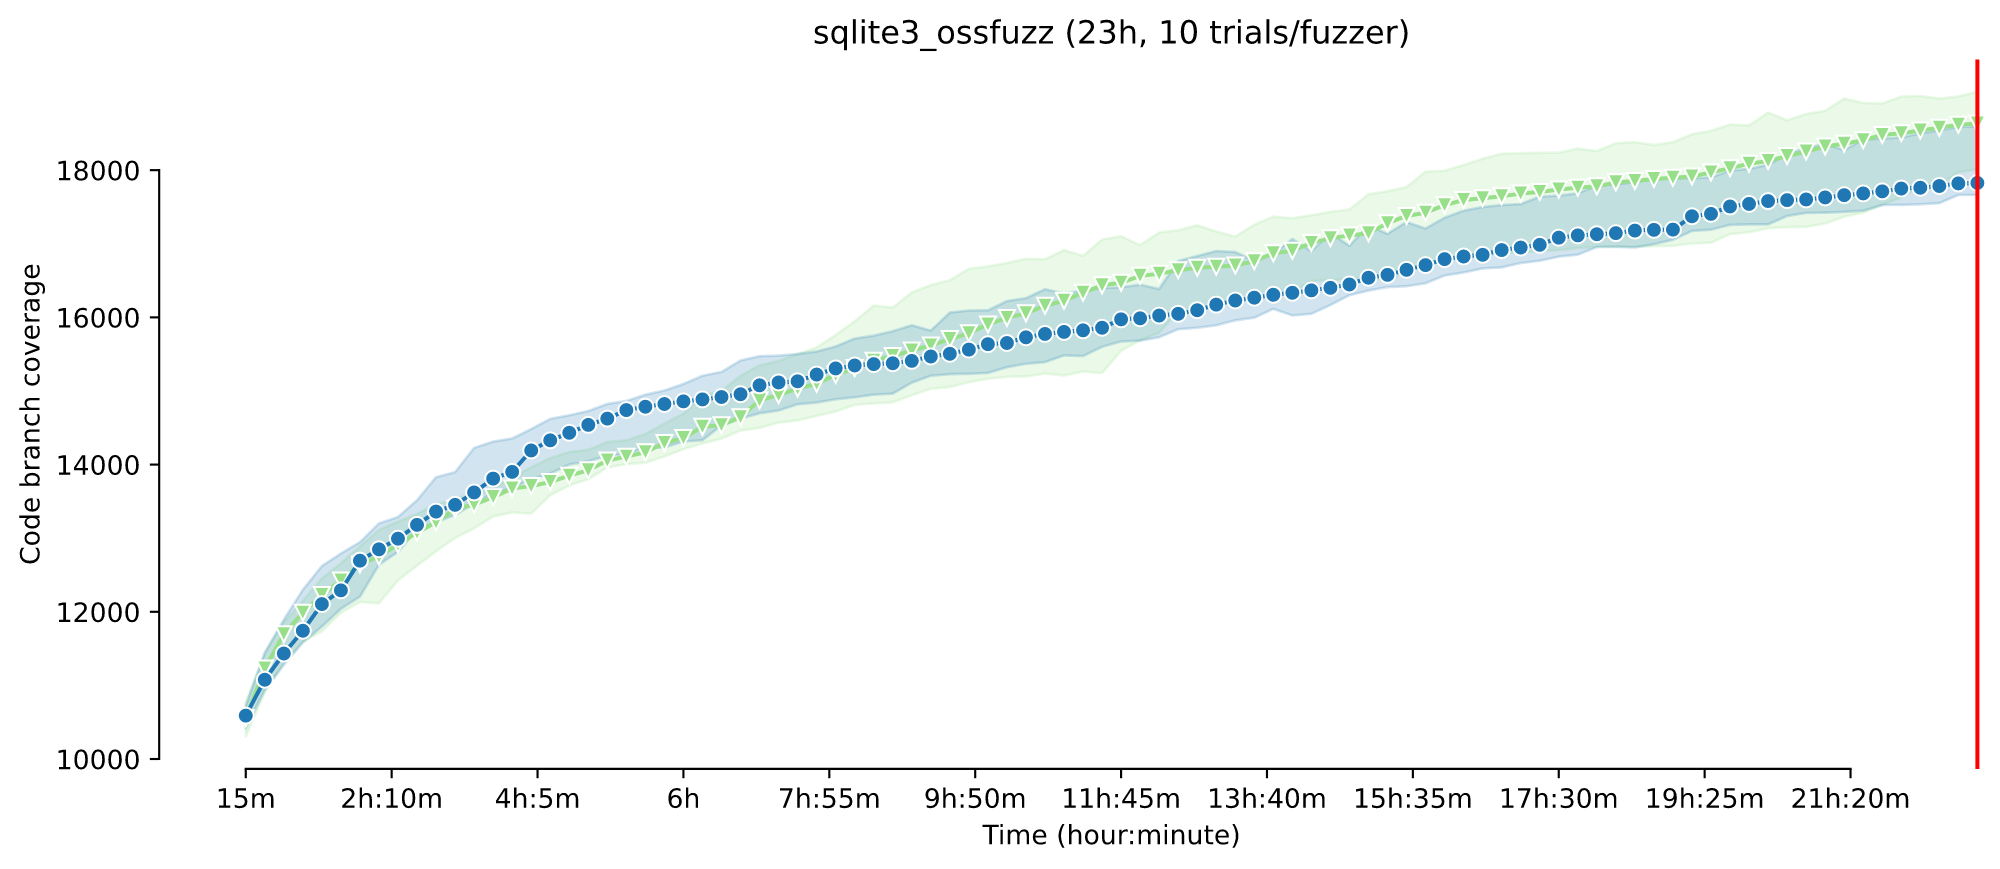
\includegraphics[width=0.65\textwidth]{assets/fuzzbench/symptr-25-vs-35-2/sqlite3_ossfuzz_coverage_growth.png}       \\
            (c) re2                                                                                                        & (d) sqlite3                                                                                                          \\[6pt]
            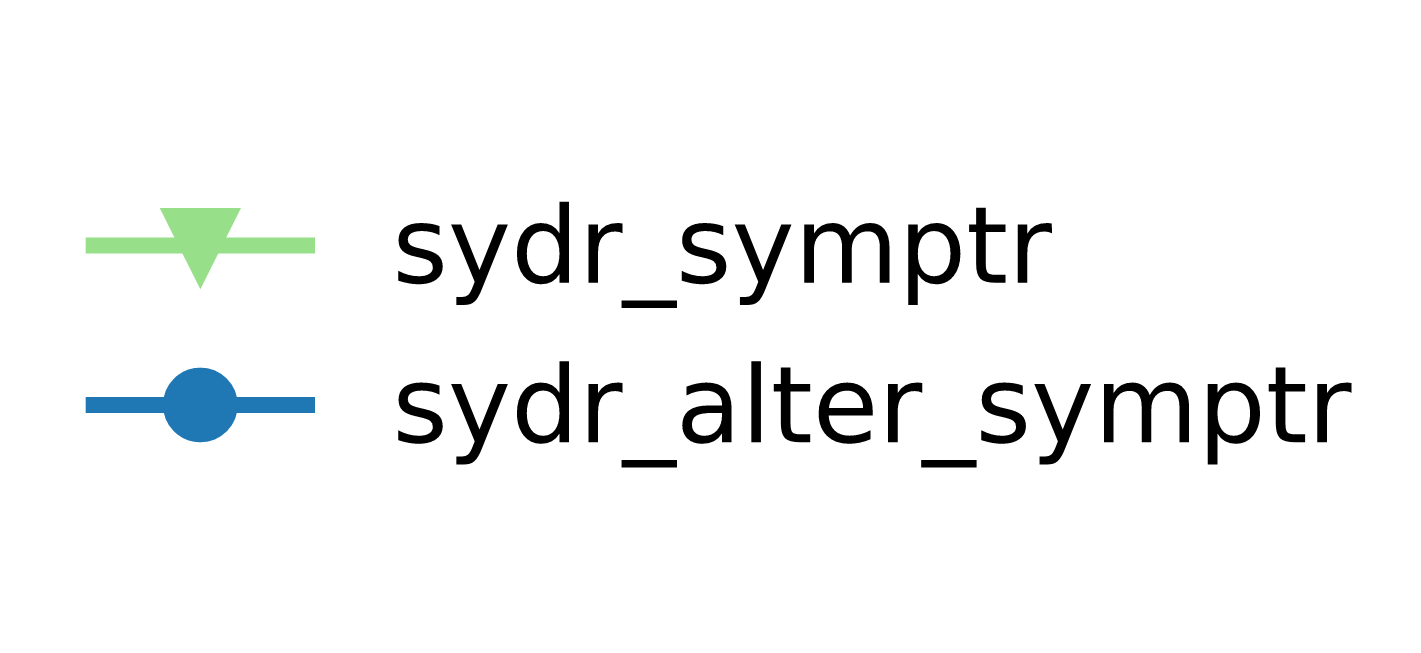
\includegraphics[width=0.65\textwidth]{assets/fuzzbench/symptr-25-vs-35-2/fuzzbench-legend.png}                &                                                                                                                      \\
            (c) legend                                                                                                     &                                                                                                                      \\[6pt]
        \end{tabular}
    }
    \caption{Fuzzbench: Symptr-25-vs-35-2 coverage growth.}
    \label{fig:fuzzbench:symptr-25-vs-35-2}
\end{figure}



\end{document}
